\documentclass[12pt]{report}
\usepackage{xcolor}
\usepackage[utf8]{inputenc}
\usepackage{natbib}
\usepackage[left=1.0in,right=1.0in,top=.8in,bottom=.8in]{geometry}
\usepackage{float}
\linespread{1.3}
\usepackage{graphicx}
\usepackage{rotating}
\usepackage{amsmath}
\usepackage{titlesec}
\usepackage{booktabs}
\usepackage{hyperref}
\usepackage{array}
\usepackage{listings}
\usepackage{longtable}

\titlespacing*{\chapter}{-15pt}{10pt}{15pt}
\titlespacing*{\section}{0pt}{5pt}{5pt}
\titlespacing*{\subsection}{0pt}{5pt}{5pt}
\titleformat{\chapter}[hang] 
{\normalfont\huge\bfseries}{\chaptertitlename\ \thechapter.}{1em}{}
\renewcommand{\chaptername}{}
\graphicspath{{Images/}}

\hypersetup{
    colorlinks=true,
    linkcolor=black,
    citecolor=blue,
    urlcolor=blue
}

\title{
{
\includegraphics[scale=.3]{logotu.jpg}}\\
\uppercase\large{
    {Tribhuvan University}\\
    {Institute of Engineering}\\
    {Pulchowk Campus}\\
    \vspace{.5cm}
    {A \\Project Report\\On\\THESIS \& PROJECT MANAGEMENT SYSTEM (TPMS)}\\
    \vspace{.5cm}
    {\textbf{Submitted By:}\\Prabesh BC (PUL080BCT054) \\Shreeyut Thapa (PUL080BCT080) \\Subesh Yadav (PUL080BCT084)}\\
    \vspace{.5cm}
    {\textbf{Submitted To:}\\ Department of Electronics \& Computer Engineering}\\
                }
    }
\date{August, 2026}

\begin{document}
\maketitle
\pagenumbering{roman}
\setcounter{page}{2}

% ── Approval Page ─────────────────────────────────────────────────────────────
\chapter*{Page of Approval}
\addcontentsline{toc}{chapter}{\numberline{}Page of Approval}
\vspace{1.5cm}
\begin{center}
\uppercase{
Tribhuvan University\\
Institute of Engineering\\
Pulchowk Campus\\
Department of Electronics and Computer Engineering
    }
\end{center}
\vspace{.5cm}
The undersigned certifies that they have read and recommended to the Institute of Engineering for acceptance of a project report entitled \textbf{"Thesis \& Project Management System (TPMS)"} submitted by \textbf{Prabesh BC (PUL080BCT054)}, \textbf{Shreeyut Thapa (PUL080BCT080)}, \textbf{Subesh Yadav (PUL080BCT084)} in partial fulfillment of the requirements for the Bachelor's degree in Computer Engineering.\\

\vspace{1.5cm}
\begin{minipage}{.5\textwidth}
    \raggedright
    .............................\\
    Supervisor\\
    \textbf{Er. Bishnu Tamang}\\
    Assistant Professor\\
    Department of Electronics and Computer Engineering,\\
    Pulchowk Campus, IOE, TU.\\
\end{minipage}%
\begin{minipage}{0.5\textwidth}
    \raggedleft
    .............................\\
    External Examiner\\
    \textbf{Dr. Kiran Mainali}\\
    Associate Professor\\
    Department of Electronics and Computer Engineering,\\
    Pulchowk Campus, IOE, TU.\\
\end{minipage}\\

\newline
\newline
\newline
\centerline{Date of approval: August 12, 2026}

% ── Copyright Page ────────────────────────────────────────────────────────────
\chapter*{Copyright}
\addcontentsline{toc}{chapter}{\numberline{}Copyright}
The author has agreed that the Library, Department of Electronics and Computer Engineering, Pulchowk Campus, and Institute of Engineering may make this report freely available for inspection. Moreover, the author has agreed that permission for extensive copying of this project report for scholarly purposes may be granted by the supervisors who supervised the work recorded herein or, in their absence, by the Head of the Department wherein the project report was done. It is understood that recognition will be given to the author of this report and the Department of Electronics and Computer Engineering, Pulchowk Campus, Institute of Engineering for any use of the material of this project report. Copying, publication, or the other use of this report for financial gain without the approval of the Department of Electronics and Computer Engineering, Pulchowk Campus, Institute of Engineering, and the author's written permission is prohibited.\\

Request for permission to copy or to make any other use of the material in this report in whole or in part should be addressed to:\\
\newline
Head\\
Department of Electronics and Computer Engineering\\
Pulchowk Campus, Institute of Engineering, TU\\
Lalitpur, Nepal.

% ── Acknowledgments ───────────────────────────────────────────────────────────
\chapter*{Acknowledgments}
\addcontentsline{toc}{chapter}{\numberline{}Acknowledgements}
We express our deepest gratitude to our project supervisor, \textbf{Er. Bishnu Tamang}, Assistant Professor at the Department of Electronics and Computer Engineering, Pulchowk Campus, for his invaluable guidance, continuous encouragement, and constructive feedback throughout the course of this project.

We extend our sincere thanks to \textbf{Prof. Dr. Sashidhar Ram Joshi}, Dean of the Institute of Engineering, and the faculty members of the Department of Electronics and Computer Engineering for providing us with the necessary infrastructure, laboratory facilities, and supportive environment.

Finally, we express our heartfelt appreciation to our fellow classmates and family members for their constant moral support and assistance throughout the development of the Thesis \& Project Management System (TPMS).

% ── Abstract ──────────────────────────────────────────────────────────────────
\chapter*{Abstract}
\addcontentsline{toc}{chapter}{\numberline{}Abstract}
The management of undergraduate projects and postgraduate theses at Pulchowk Campus, Institute of Engineering (IOE), has traditionally relied on fragmented manual workflows, paper evaluation sheets, and uncoordinated email communications. This manual paradigm leads to supervision tracking opacity, administrative bottlenecks during evaluation periods, and error-prone mark aggregation. To address these systemic inefficiencies, we present the \textbf{Thesis \& Project Management System (TPMS)}, a comprehensive, secure, multi-tier web platform tailored specifically to the academic governance structures of Pulchowk Campus.

TPMS integrates five distinct role-based access levels—Student, Supervisor, External Examiner, Program Coordinator, and Maintainer—across six academic degree programs (BCT, BEI, MSNCS, MSICE, MSDSA, MSCSKE). Built upon a modern React 18 single-page application frontend and a Node.js Express REST API backend connected to a PostgreSQL database via Prisma ORM, TPMS encapsulates the complete project lifecycle: group formation, bulk Excel student importing with anomaly detection, supervisor assignment, document submission, and criteria-based evaluation.

Crucially, TPMS features a headless \textbf{Puppeteer PDF rendering engine} that dynamically compiles official, university-branded A4 evaluation sheets with automatic word-to-number mark conversion, as well as an auxiliary \textbf{Retrieval-Augmented Generation (RAG) AI Chatbot microservice} (built with FastAPI, ChromaDB, and Llama-3/Gemini) that offers real-time proposal analysis and guidelines QA. Rigorous empirical validation demonstrates 100\% mark calculation accuracy, instantaneous PDF generation under 1.2 seconds, and seamless scaling across multi-batch academic rosters.\\

\newline
Keywords: \textit{Academic Management, Thesis Governance, Role-Based Access Control, Headless PDF Rendering, Retrieval-Augmented Generation, React, Node.js, Prisma ORM, PostgreSQL}

% ── Tables & Lists ────────────────────────────────────────────────────────────
\tableofcontents
\addcontentsline{toc}{chapter}{\numberline{}Contents}
\listoffigures
\addcontentsline{toc}{chapter}{\numberline{}List of Figures}
\listoftables
\addcontentsline{toc}{chapter}{\numberline{}List of Tables}

\chapter*{List of Abbreviations}
\addcontentsline{toc}{chapter}{\numberline{}List of Abbreviations}
\begin{tabular}{c l}
\textbf{API}      & Application Programming Interface\\
\textbf{BCT}      & Bachelor in Computer Engineering\\
\textbf{BEI}      & Bachelor in Electronics, Communication \& Information Engineering\\
\textbf{CORS}     & Cross-Origin Resource Sharing\\
\textbf{DFD}      & Data Flow Diagram\\
\textbf{DOECE}    & Department of Electronics and Computer Engineering\\
\textbf{ER}       & Entity-Relationship\\
\textbf{IOE}      & Institute of Engineering\\
\textbf{JWT}      & JSON Web Token\\
\textbf{ORM}      & Object-Relational Mapping\\
\textbf{PDF}      & Portable Document Format\\
\textbf{RAG}      & Retrieval-Augmented Generation\\
\textbf{REST}     & Representational State Transfer\\
\textbf{SPA}      & Single Page Application\\
\textbf{TPMS}     & Thesis \& Project Management System\\
\textbf{TU}       & Tribhuvan University\\
\textbf{UI}       & User Interface\\
\textbf{URL}      & Uniform Resource Locator
\end{tabular}

% ── CHAPTER 1: INTRODUCTION ───────────────────────────────────────────────────
\chapter{Introduction}
\pagenumbering{arabic}

\section{Background}
Academic project work and thesis research represent the pinnacle of engineering education at Pulchowk Campus, Institute of Engineering (IOE), Tribhuvan University. For undergraduate programs such as Bachelor in Computer Engineering (BCT) and Bachelor in Electronics, Communication \& Information Engineering (BEI), students complete Minor Projects (in their 3rd year) and Major Projects (in their 4th year). Concurrently, postgraduate students across Master of Science programs (MSNCS, MSICE, MSDSA, MSCSKE) undergo rigorous thesis research spanning proposal defense, mid-term evaluation, and final defense.

Despite the high technical caliber of research produced, the administrative orchestration of these academic activities has historically relied on physical paper evaluation sheets, manual group registration forms, notice board announcements, and uncoordinated email exchanges. Departmental program coordinators face severe logistical overhead when managing hundreds of enrolled students, mapping project groups to eligible supervisors, distributing evaluation rubrics to external examiners, and compiling physical marks into final grade sheets.

Modern web engineering techniques combined with automated document compilation offer an ideal solution to digitalize academic administration. The Thesis \& Project Management System (TPMS) was conceived to replace paper-bound bottlenecks with a unified, transparent, and resilient digital platform engineered specifically for IOE DOECE standards \citep{pressman2014software}.

\section{Problem Statement}
The legacy paper-based project and thesis management workflow at Pulchowk Campus exhibits several critical operational drawbacks:
\begin{enumerate}
    \item \textbf{High Administrative Burden:} Program coordinators manually track student groups, check roll number validity, verify project titles, and match student groups with available faculty supervisors using physical lists.
    \item \textbf{Supervision \& Progress Opacity:} Students and department heads lack real-time visibility into supervisor assignment status, recommendation status, and evaluation schedules.
    \item \textbf{Error-Prone Evaluation Sheet Compilation:} Supervisors and external examiners manually write numerical marks, convert total scores into words, and submit physical evaluation sheets. Manual calculations frequently introduce transcription errors and delays in forwarding results to the exam section.
    \item \textbf{Document Versioning Disarray:} Project proposals, progress reports, and thesis manuscripts are exchanged via scattered email attachments, resulting in loss of submission histories and lack of automated proposal review tools.
\end{enumerate}

\section{Objectives}
The primary objective of this project is to design, develop, test, and deploy a secure, web-based Thesis \& Project Management System (TPMS) customized for Pulchowk Campus, IOE. The specific sub-objectives are:
\begin{itemize}
    \item To implement a granular 5-role security model (Student, Supervisor, External Examiner, Program Coordinator, Maintainer) with role-specific navigation and program-scoped data access.
    \item To build an automated Excel batch import module capable of parsing class rosters, identifying data anomalies, and auto-provisioning student groups and supervisor assignments.
    \item To develop an interactive evaluation workbench with criteria-based mark entry, real-time total score calculation, and word-equivalent mark transformation.
    \item To integrate a server-side Puppeteer PDF rendering engine that generates official, university-formatted A4 evaluation sheets ready for digital signature and printing.
    \item To implement a Retrieval-Augmented Generation (RAG) AI Chatbot microservice to assist students with proposal guideline queries and document analysis.
\end{itemize}

\section{Scope \& Limitations}
The scope of TPMS encompasses the academic administration of Minor/Major projects for BCT and BEI programs, as well as Master thesis workflows for MSNCS, MSICE, MSDSA, and MSCSKE programs within the DOECE department.

\textbf{Limitations:}
\begin{itemize}
    \item The current release focuses on departmental governance within DOECE and requires administrative authorization for campus-wide integration across other engineering departments.
    \item Digital signature verification relies on physical printing or PDF approval tokens rather than PKI hardware tokens.
\end{itemize}

% ── CHAPTER 2: LITERATURE REVIEW ──────────────────────────────────────────────
\chapter{Literature Review}

\section{Related Work}
Digital transformation in higher education administration has driven the adoption of Learning Management Systems (LMS) such as Moodle and Canvas, alongside specialized thesis repository systems like DSpace. However, commercial LMS platforms primarily target course content delivery, quizzes, and gradebooks, failing to model complex academic project workflows—such as multi-student group formation, dual external examiner assignment, 5-criteria rubric evaluation, and institutional grade forwarding.

Prior work by \citet{giri2019transfer} highlighted the necessity of domain-specific academic workflow automation in Nepali engineering institutions. Existing open-source portals often lack native PDF template compilation adhering to official university evaluation sheets (such as IOE Pulchowk Campus formats), forcing faculty to manually transcribe digital grades back onto paper forms.

\section{Related Theory}

\subsection{Single-Page Application (SPA) Architecture}
Modern web applications leverage SPA patterns, where the web browser loads a single HTML shell and dynamically updates content via RESTful API calls without full page reloads. React 18, utilizing a virtual DOM and concurrent rendering, enables highly reactive UI updates essential for multi-criteria evaluation workbenches.

\subsection{RESTful API & JWT Authentication}
Representational State Transfer (REST) provides a scalable client-server architectural style \citep{fielding2000architectural}. Statutory authentication in stateless REST APIs is achieved via JSON Web Tokens (JWT). A JWT consists of a base64-encoded Header, Payload (containing user ID, role, and program scope), and a cryptographic Signature verified using HMAC-SHA256.

\subsection{Object-Relational Mapping (ORM) with Prisma}
Database access in node.js applications has evolved from raw SQL queries to type-safe ORM layers. Prisma 5 utilizes a declarative schema specification (`schema.prisma`) to auto-generate TypeScript/JavaScript client bindings, enforcing foreign key integrity, schema migrations, and relational eager loading across complex entities.

\subsection{Server-Side Headless PDF Generation}
Compiling dynamic HTML templates into print-ready A4 PDF documents requires headless browser execution. Puppeteer controls headless Chromium via the Chrome DevTools Protocol, executing pixel-perfect CSS Paged Media layout algorithms (`@page { size: A4; margin: 15mm; }`) to render university headers, logos, and signatures.

\subsection{Retrieval-Augmented Generation (RAG)}
Large Language Models (LLMs) can suffer from factual hallucination when queried on specific institutional guidelines. Retrieval-Augmented Generation \citep{lewis2020retrieval} mitigates this by embedding domain documents into a dense vector space using vector databases like ChromaDB. When a user submits a query, semantic similarity search retrieves the top-$k$ relevant text chunks, which are prepended into the LLM context prompt to generate verified answers.

% ── CHAPTER 3: METHODOLOGY ────────────────────────────────────────────────────
\chapter{Methodology}

\section{Requirement Analysis & Feasibility Study}
The methodology commenced with a comprehensive requirement gathering phase involving interviews with DOECE program coordinators, project supervisors, and final-year BCT students at Pulchowk Campus.

\textbf{Functional Requirements:}
\begin{itemize}
    \item \textbf{FR1 (Authentication):} Secure login with role determination and password hashing (bcryptjs).
    \item \textbf{FR2 (Group Formation):} Student-initiated group creation with invitation confirmation and roll number validation.
    \item \textbf{FR3 (Bulk Import):} Excel file upload (.xlsx) by coordinators to auto-create groups and assign faculty.
    \item \textbf{FR4 (Evaluation Workbench):} Rubric-based scoring (5 criteria $\times$ 20 marks = 100 total) for Supervisor, Mid-Term External, and Final External evaluators.
    \item \textbf{FR5 (PDF Generation):} Automated creation of official IOE evaluation sheets.
    \item \textbf{FR6 (AI Assistance):} RAG-driven chatbot for proposal QA.
\end{itemize}

\textbf{Technical Feasibility:} The chosen technology stack—React 18, Node.js 18, Express, PostgreSQL 16, Prisma 5, Puppeteer, and FastAPI—consists entirely of open-source, enterprise-grade frameworks supported on Linux environments.

\section{Software Development Lifecycle (Agile Workflow)}
The system was developed following an Agile Scrum methodology over a 16-week timeline, divided into four 4-week sprints:
\begin{itemize}
    \item \textbf{Sprint 1:} Database schema design, Prisma ORM migration, JWT authentication, and user management endpoints.
    \item \textbf{Sprint 2:} Student group formation, proposal upload, and coordinator management dashboards.
    \item \textbf{Sprint 3:} Evaluation workbench, Puppeteer PDF rendering engine, and Excel bulk import module.
    \item \textbf{Sprint 4:} FastAPI RAG AI chatbot microservice integration, system testing, and security hardening.
\end{itemize}

\section{Data Model Design}
The relational database was modeled in PostgreSQL via Prisma ORM, consisting of 18 schema entities. Key relationships include:
\begin{itemize}
    \item `User` (1) $\rightarrow$ (1) `Student` or (1) `Faculty`
    \item `Group` (1) $\rightarrow$ ($N$) `Student`, (1) $\rightarrow$ (1) `Project`
    \item `Project` (1) $\rightarrow$ ($N$) `Proposal`, (1) $\rightarrow$ ($N$) `SupervisorAssignment`
    \item `Project` (1) $\rightarrow$ ($N$) `Evaluation` $\rightarrow$ ($N$) `CriterionMark`
\end{itemize}

\section{Security & Role-Based Access Control (RBAC)}
Security is enforced at both API gateway and database query levels. Express middleware inspects incoming `Authorization: Bearer <token>` headers:
\begin{lstlisting}[language=Java, caption={JWT RBAC Middleware Snippet}]
const authorize = (allowedRoles = []) => {
  return (req, res, next) => {
    if (!req.user || !allowedRoles.includes(req.user.role)) {
      return res.status(403).json({ error: "Access Denied" });
    }
    next();
  };
};
\end{lstlisting}

% ── CHAPTER 4: SYSTEM DESIGN ──────────────────────────────────────────────────
\chapter{System Design}

\section{System Architecture}
TPMS utilizes a 4-tier decoupled software architecture designed for high availability, security, and computational separation, as illustrated in Figure \ref{fig:sys_arch}.

\begin{figure}[H]
    \centering
    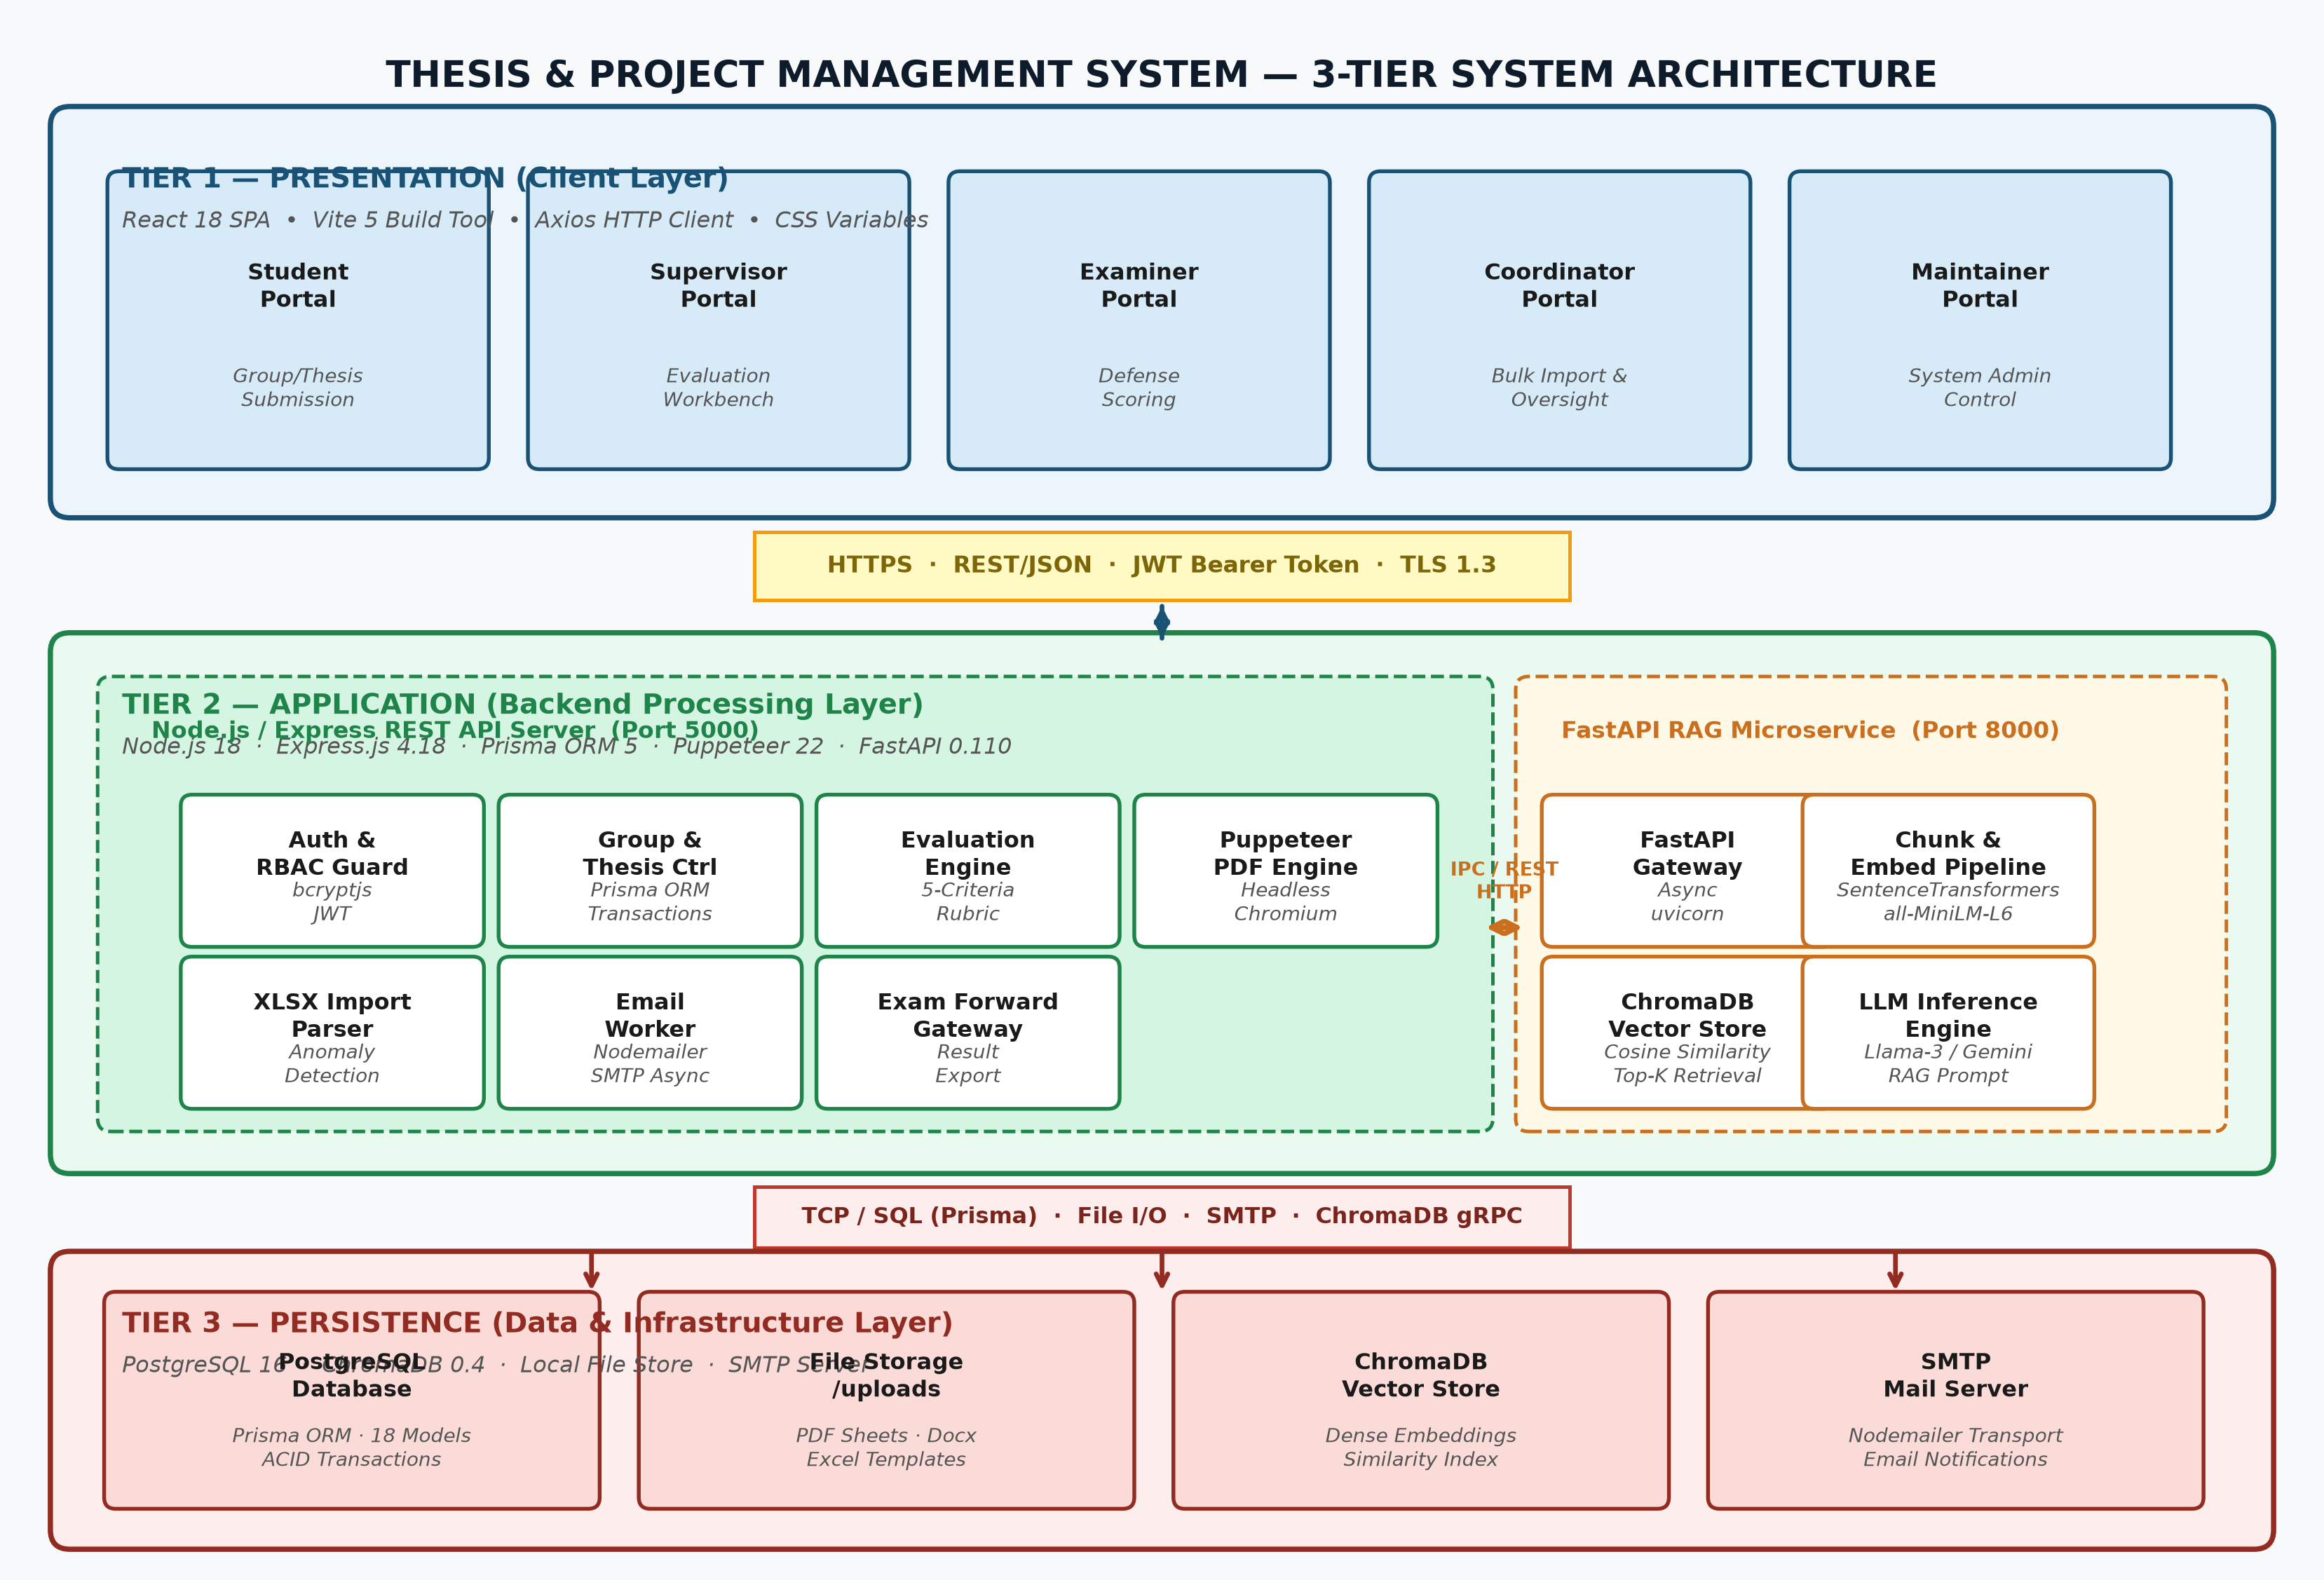
\includegraphics[width=0.98\textwidth]{fig_1_system_architecture.png}
    \caption{Thesis \& Project Management System (TPMS) System Architecture}
    \label{fig:sys_arch}
\end{figure}

The layers comprise:
\begin{enumerate}
    \item \textbf{Presentation Tier:} React 18 SPA serving responsive interfaces for 5 user roles.
    \item \textbf{API Gateway & Core Application Tier:} Node.js/Express server orchestrating REST endpoints, JWT authorization, Puppeteer PDF rendering, and Excel parsing.
    \item \textbf{AI Microservice Tier:} FastAPI service housing the ChromaDB vector store and RAG pipeline.
    \item \textbf{Persistence Tier:} PostgreSQL 16 relational database, local file storage (`/uploads`), and Nodemailer SMTP mail gateway.
\end{enumerate}

\section{Module Breakdown}
TPMS is divided into seven core functional modules:
\begin{itemize}
    \item \textbf{Auth Module:} User registration, password hashing, JWT token issuance.
    \item \textbf{Group Module:} Group formation, student invitations, academic year filter.
    \item \textbf{Import Module:} Excel file parser (`xlsx`), roll number verification, anomaly detection preview.
    \item \textbf{Evaluation Module:} Dynamic rubric loader, numerical entry, automated grade calculation.
    \item \textbf{Print Engine:} Puppeteer HTML-to-PDF compiler for university A4 evaluation sheets.
    \item \textbf{AI Chatbot Module:} Vector search retriever and LLM answer generator.
    \item \textbf{Exam Forwarding Module:} Result consolidation and section transfer.
\end{itemize}

\section{Use Case Analysis}
The interactions between system actors and core use cases are depicted in Figure \ref{fig:use_case}.

\begin{figure}[H]
    \centering
    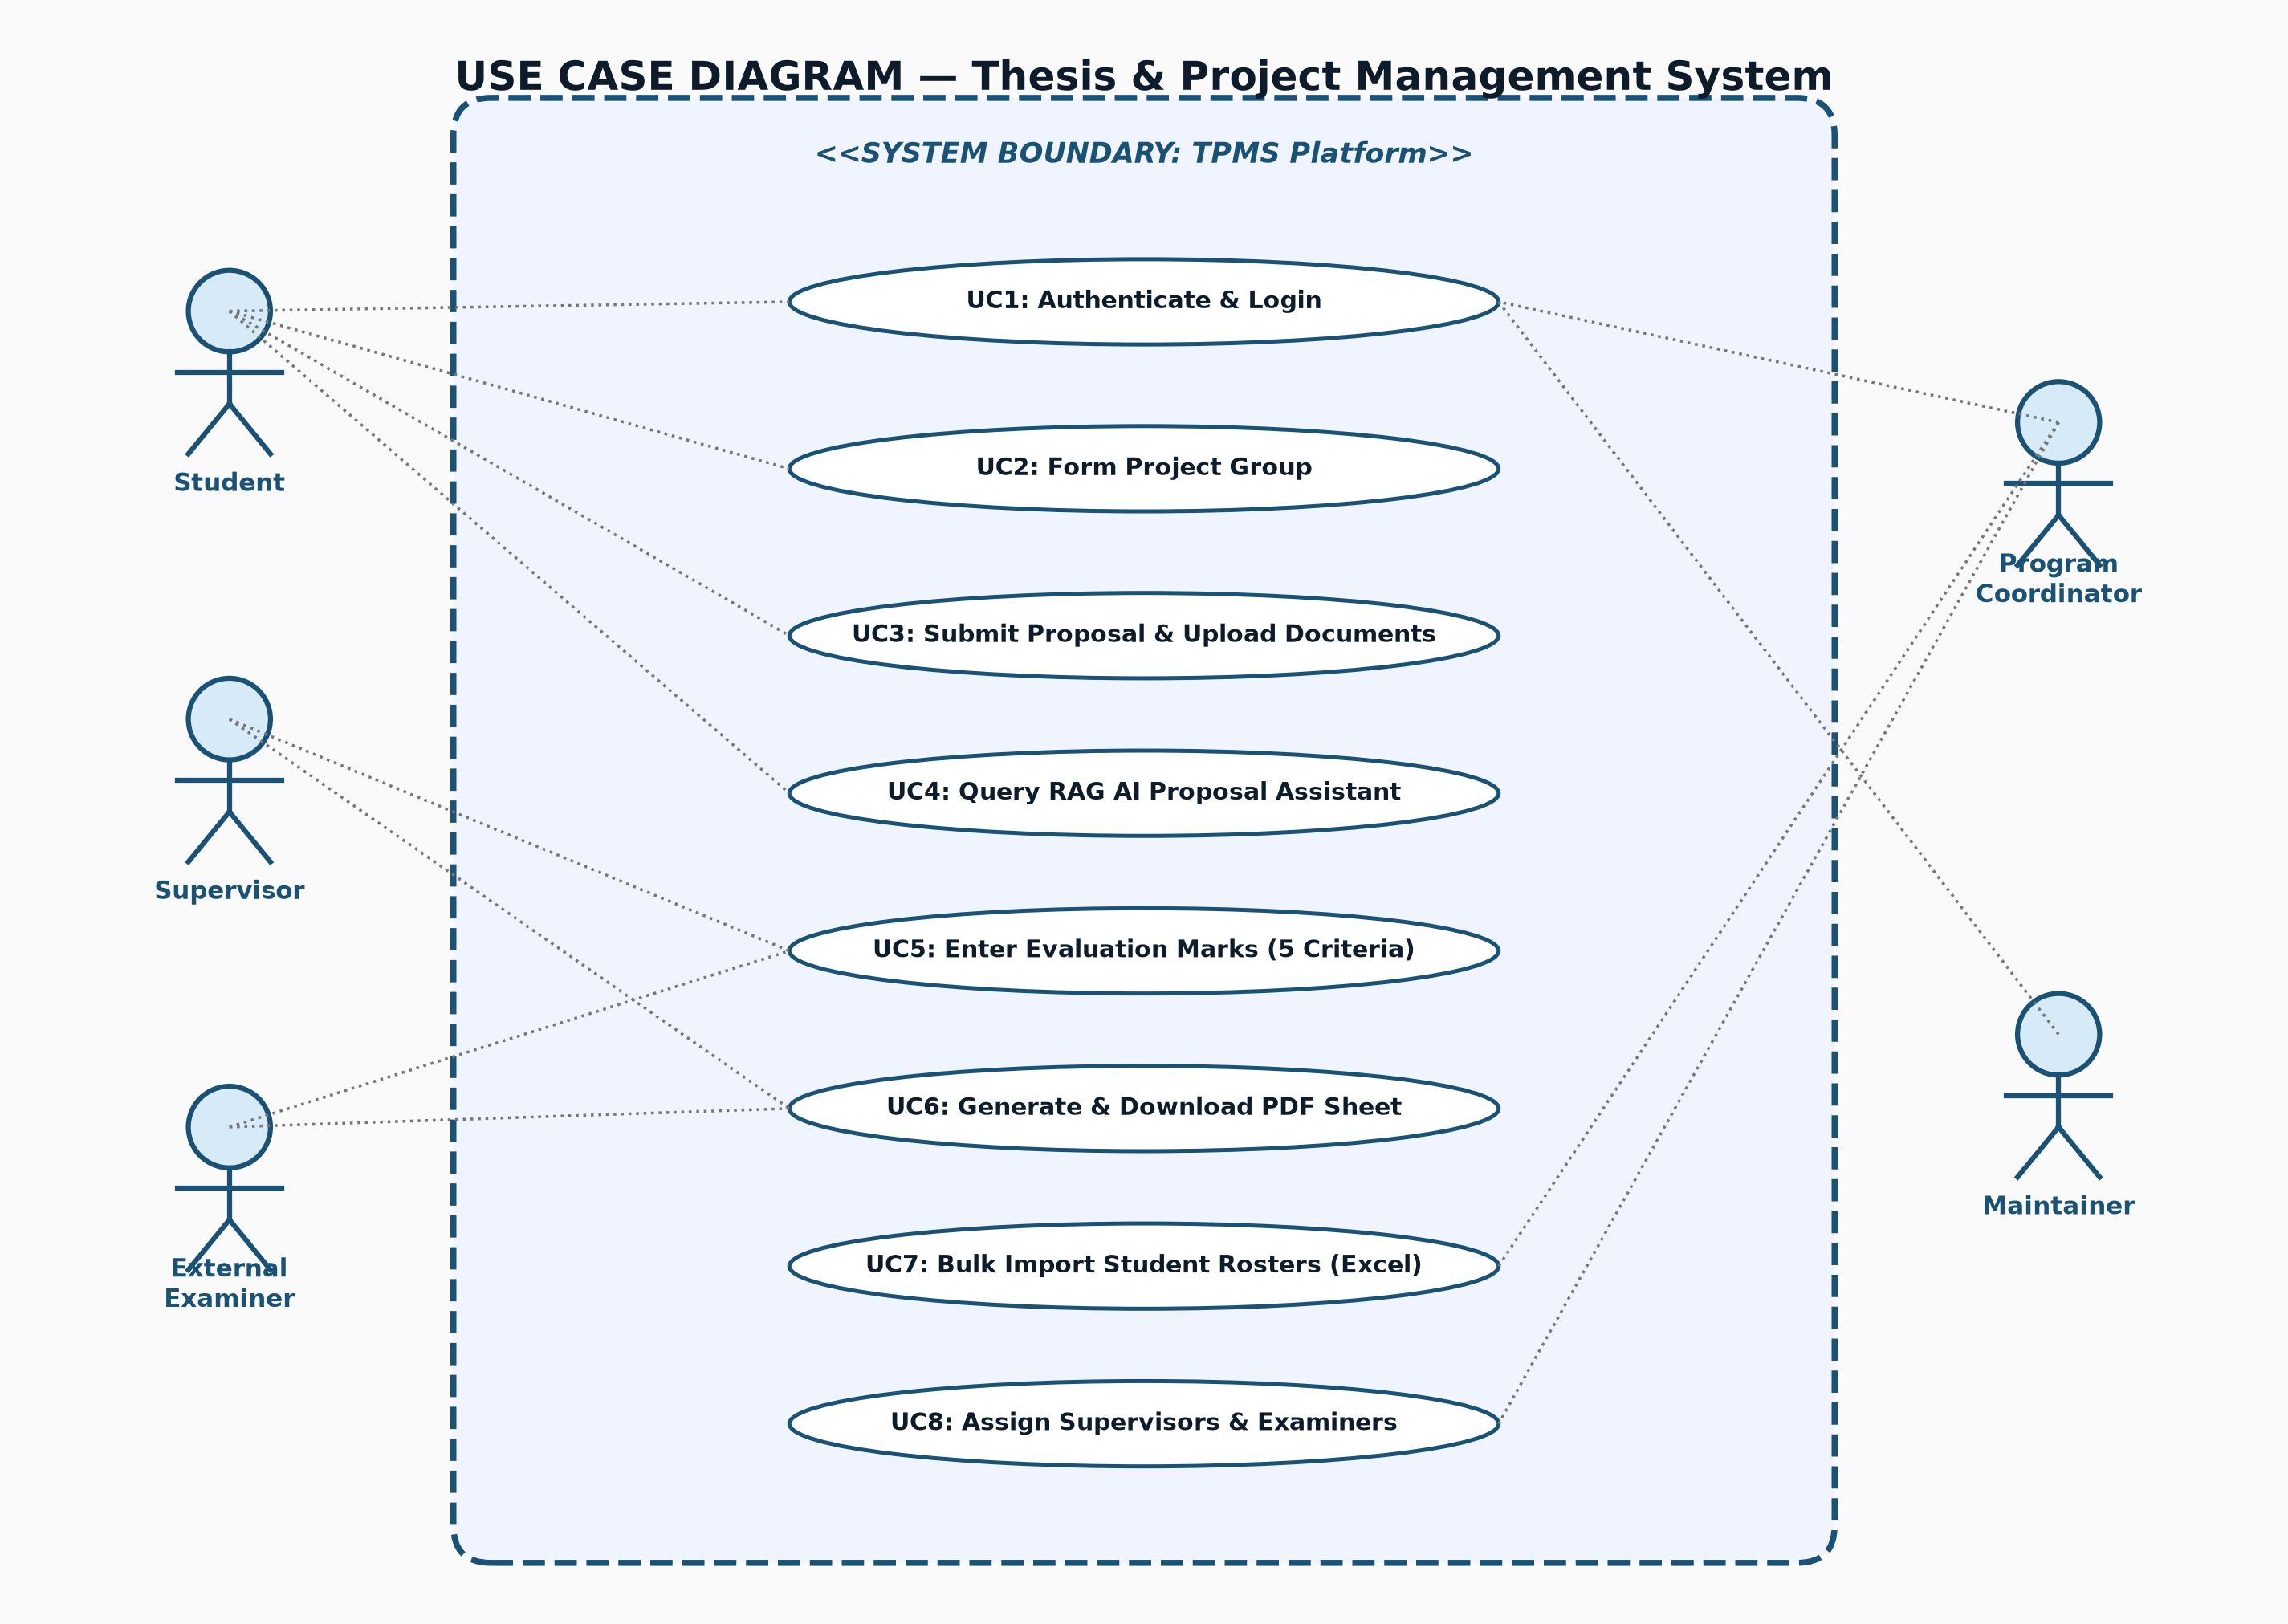
\includegraphics[width=0.92\textwidth]{fig_2_use_case_diagram.png}
    \caption{TPMS Use Case Diagram}
    \label{fig:use_case}
\end{figure}

\section{Entity-Relationship (ER) Diagram}
The relational database structure comprising 18 entities and foreign key constraints is shown in Figure \ref{fig:er_diagram}.

\begin{figure}[H]
    \centering
    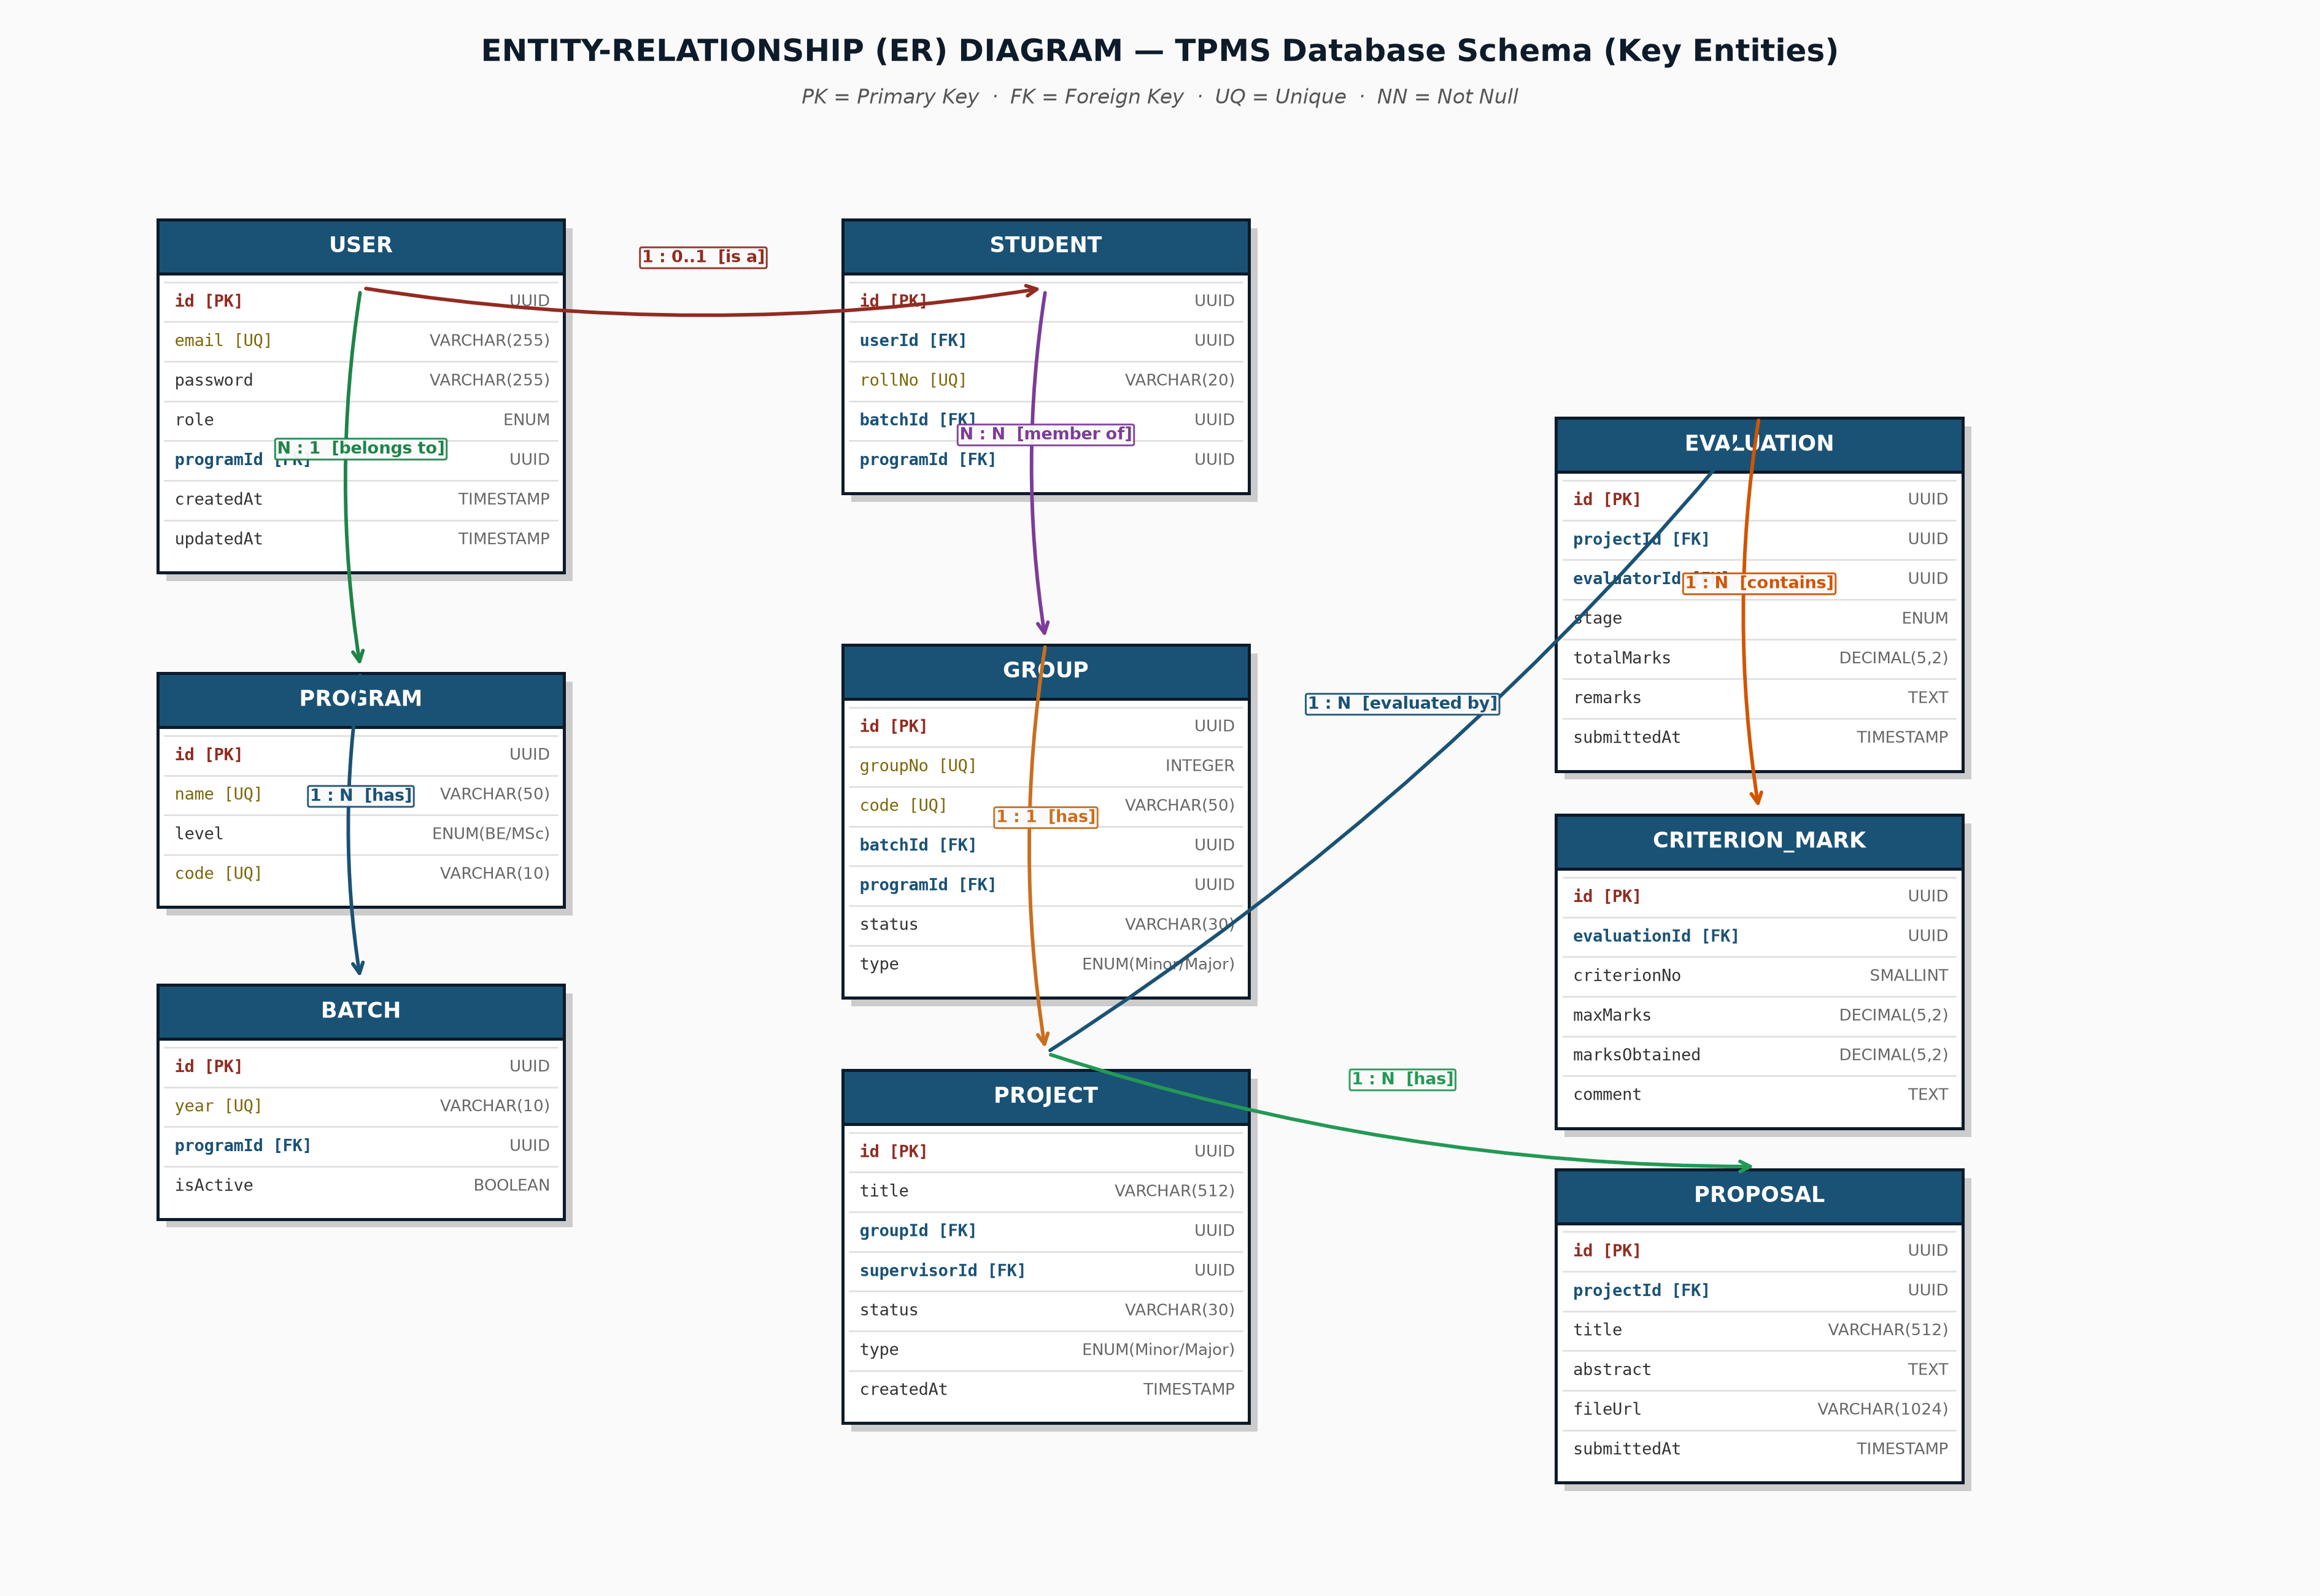
\includegraphics[width=0.95\textwidth]{fig_3_er_diagram.png}
    \caption{Entity-Relationship (ER) Diagram}
    \label{fig:er_diagram}
\end{figure}

\section{Data Flow Diagram (DFD Level 1)}
The high-level data transformation pipelines between external actors, processing nodes, and data stores are presented in Figure \ref{fig:dfd1}.

\begin{figure}[H]
    \centering
    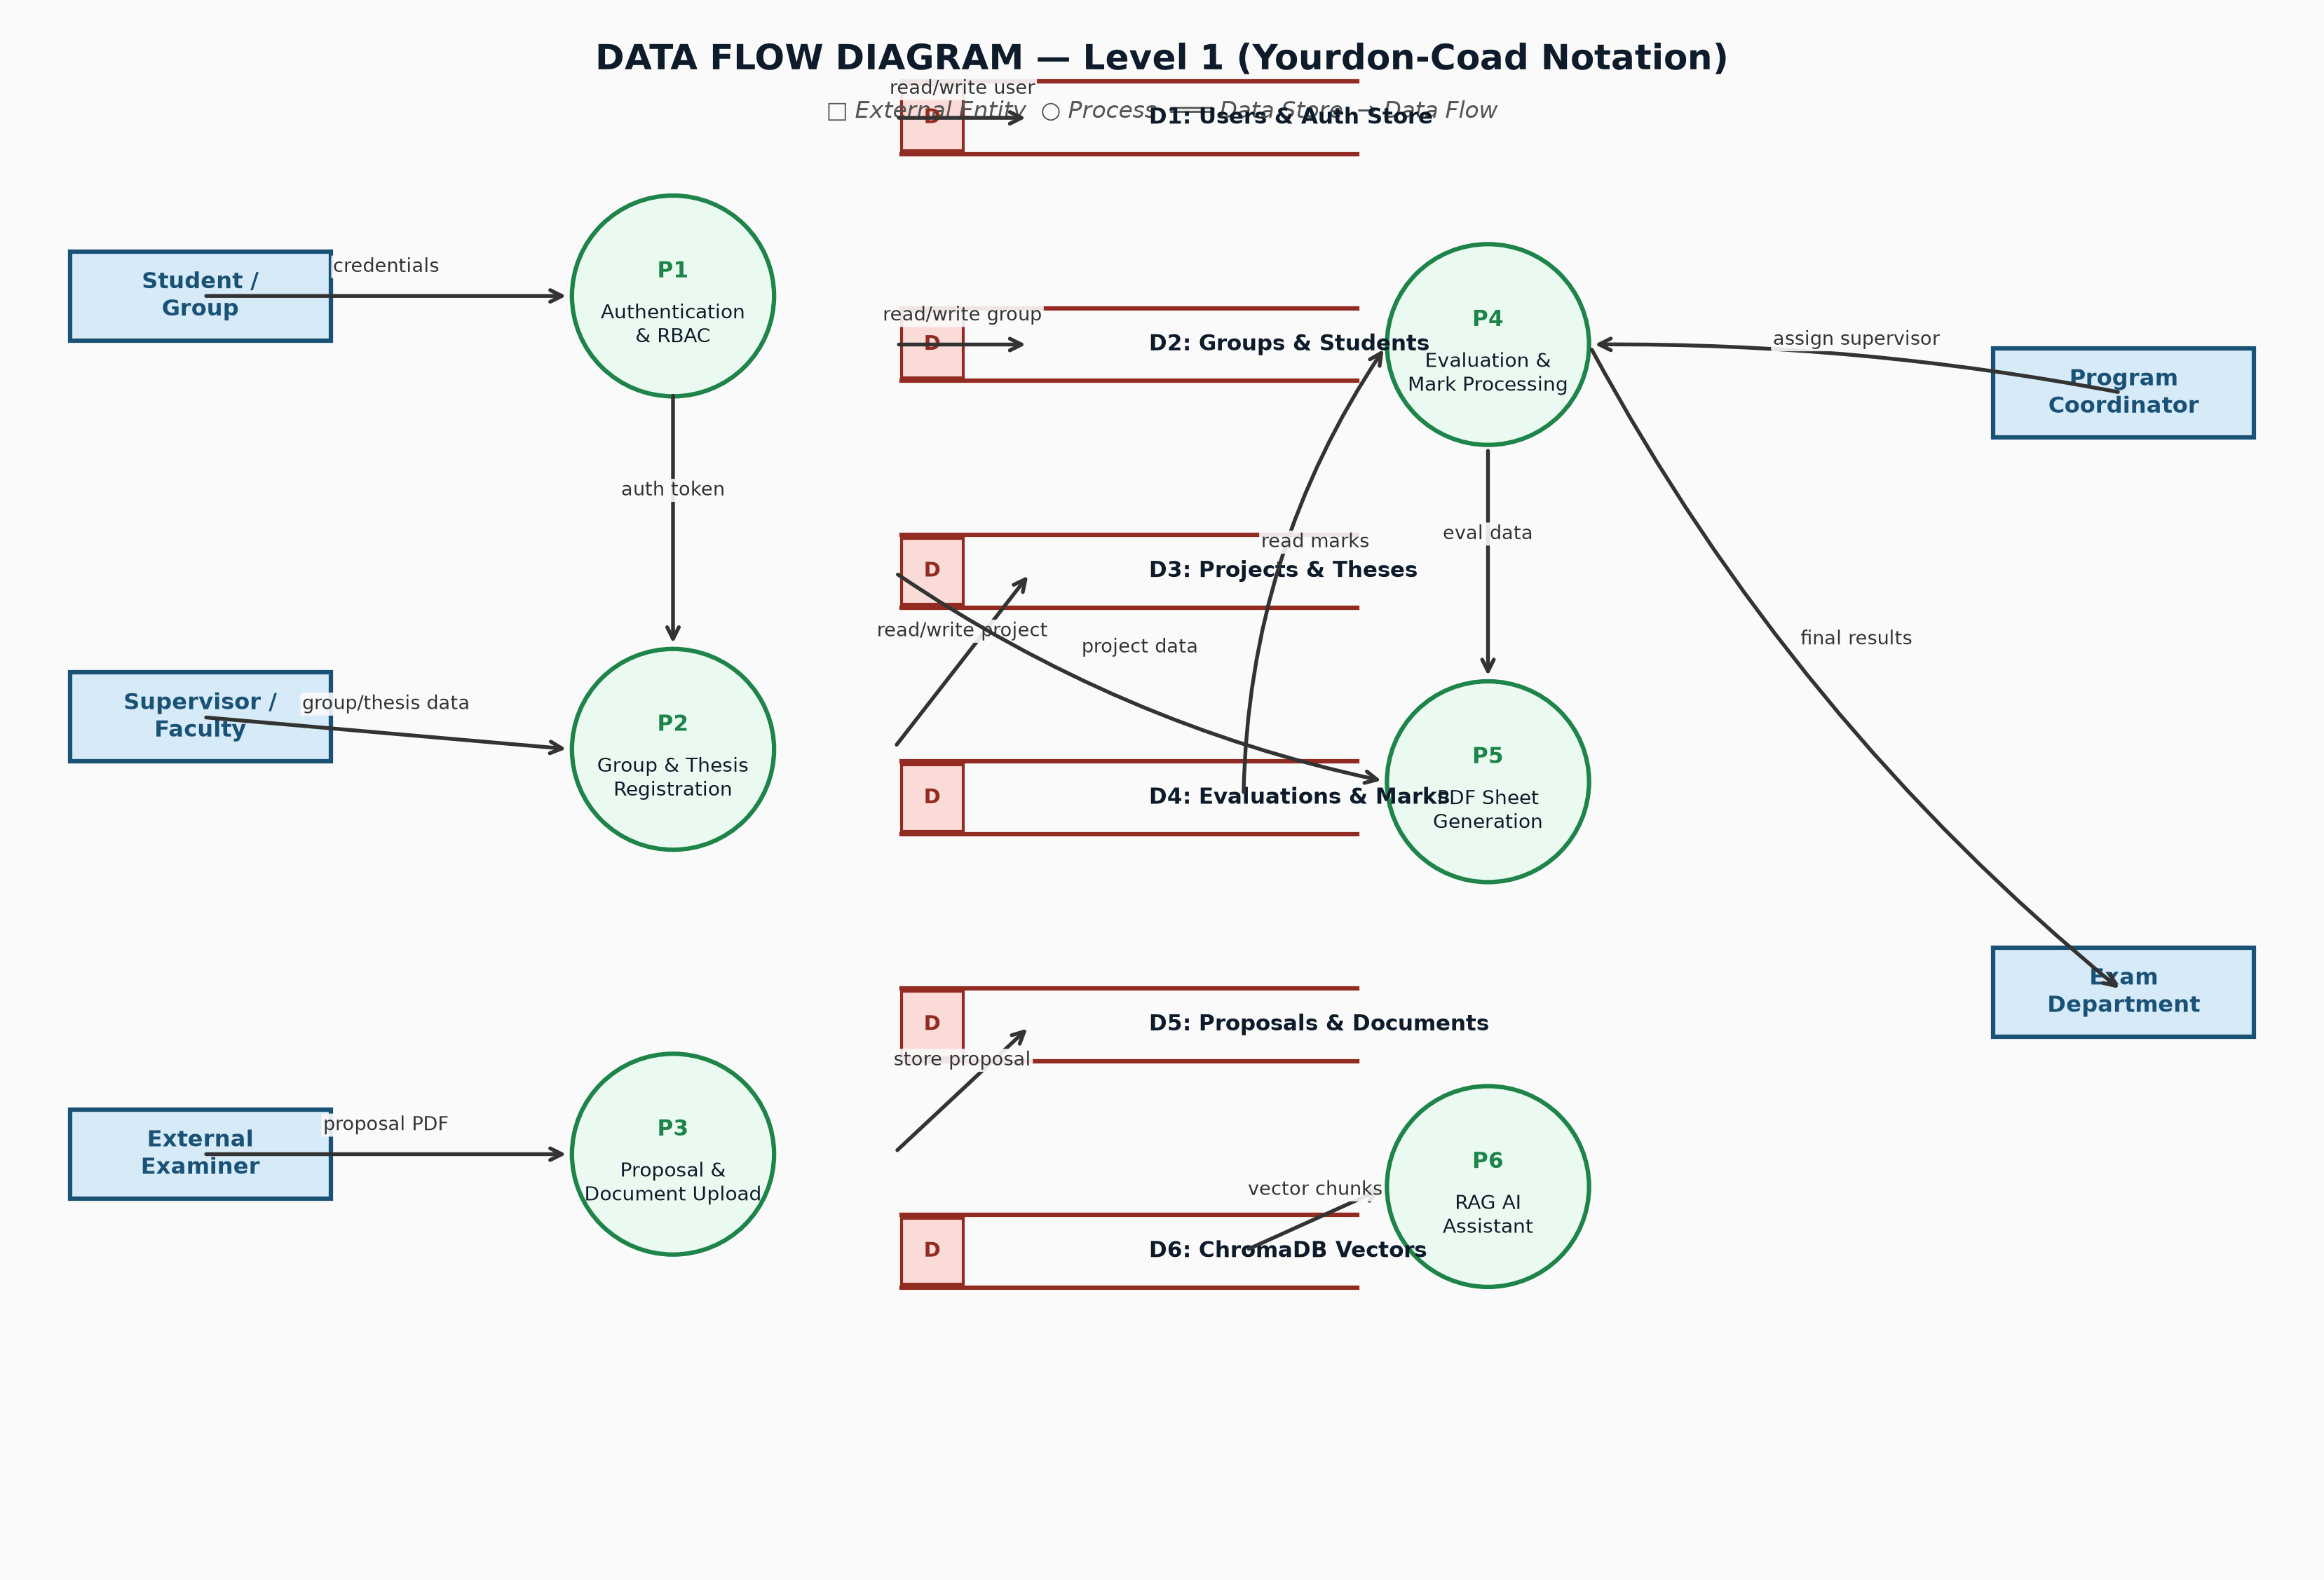
\includegraphics[width=0.92\textwidth]{fig_7_dfd_level_1.png}
    \caption{Data Flow Diagram (DFD Level 1)}
    \label{fig:dfd1}
\end{figure}

\section{Sequence Diagrams}
Figures \ref{fig:seq_import}, \ref{fig:seq_assign}, and \ref{fig:seq_eval} illustrate the dynamic control flows for critical system operations.

\begin{figure}[H]
    \centering
    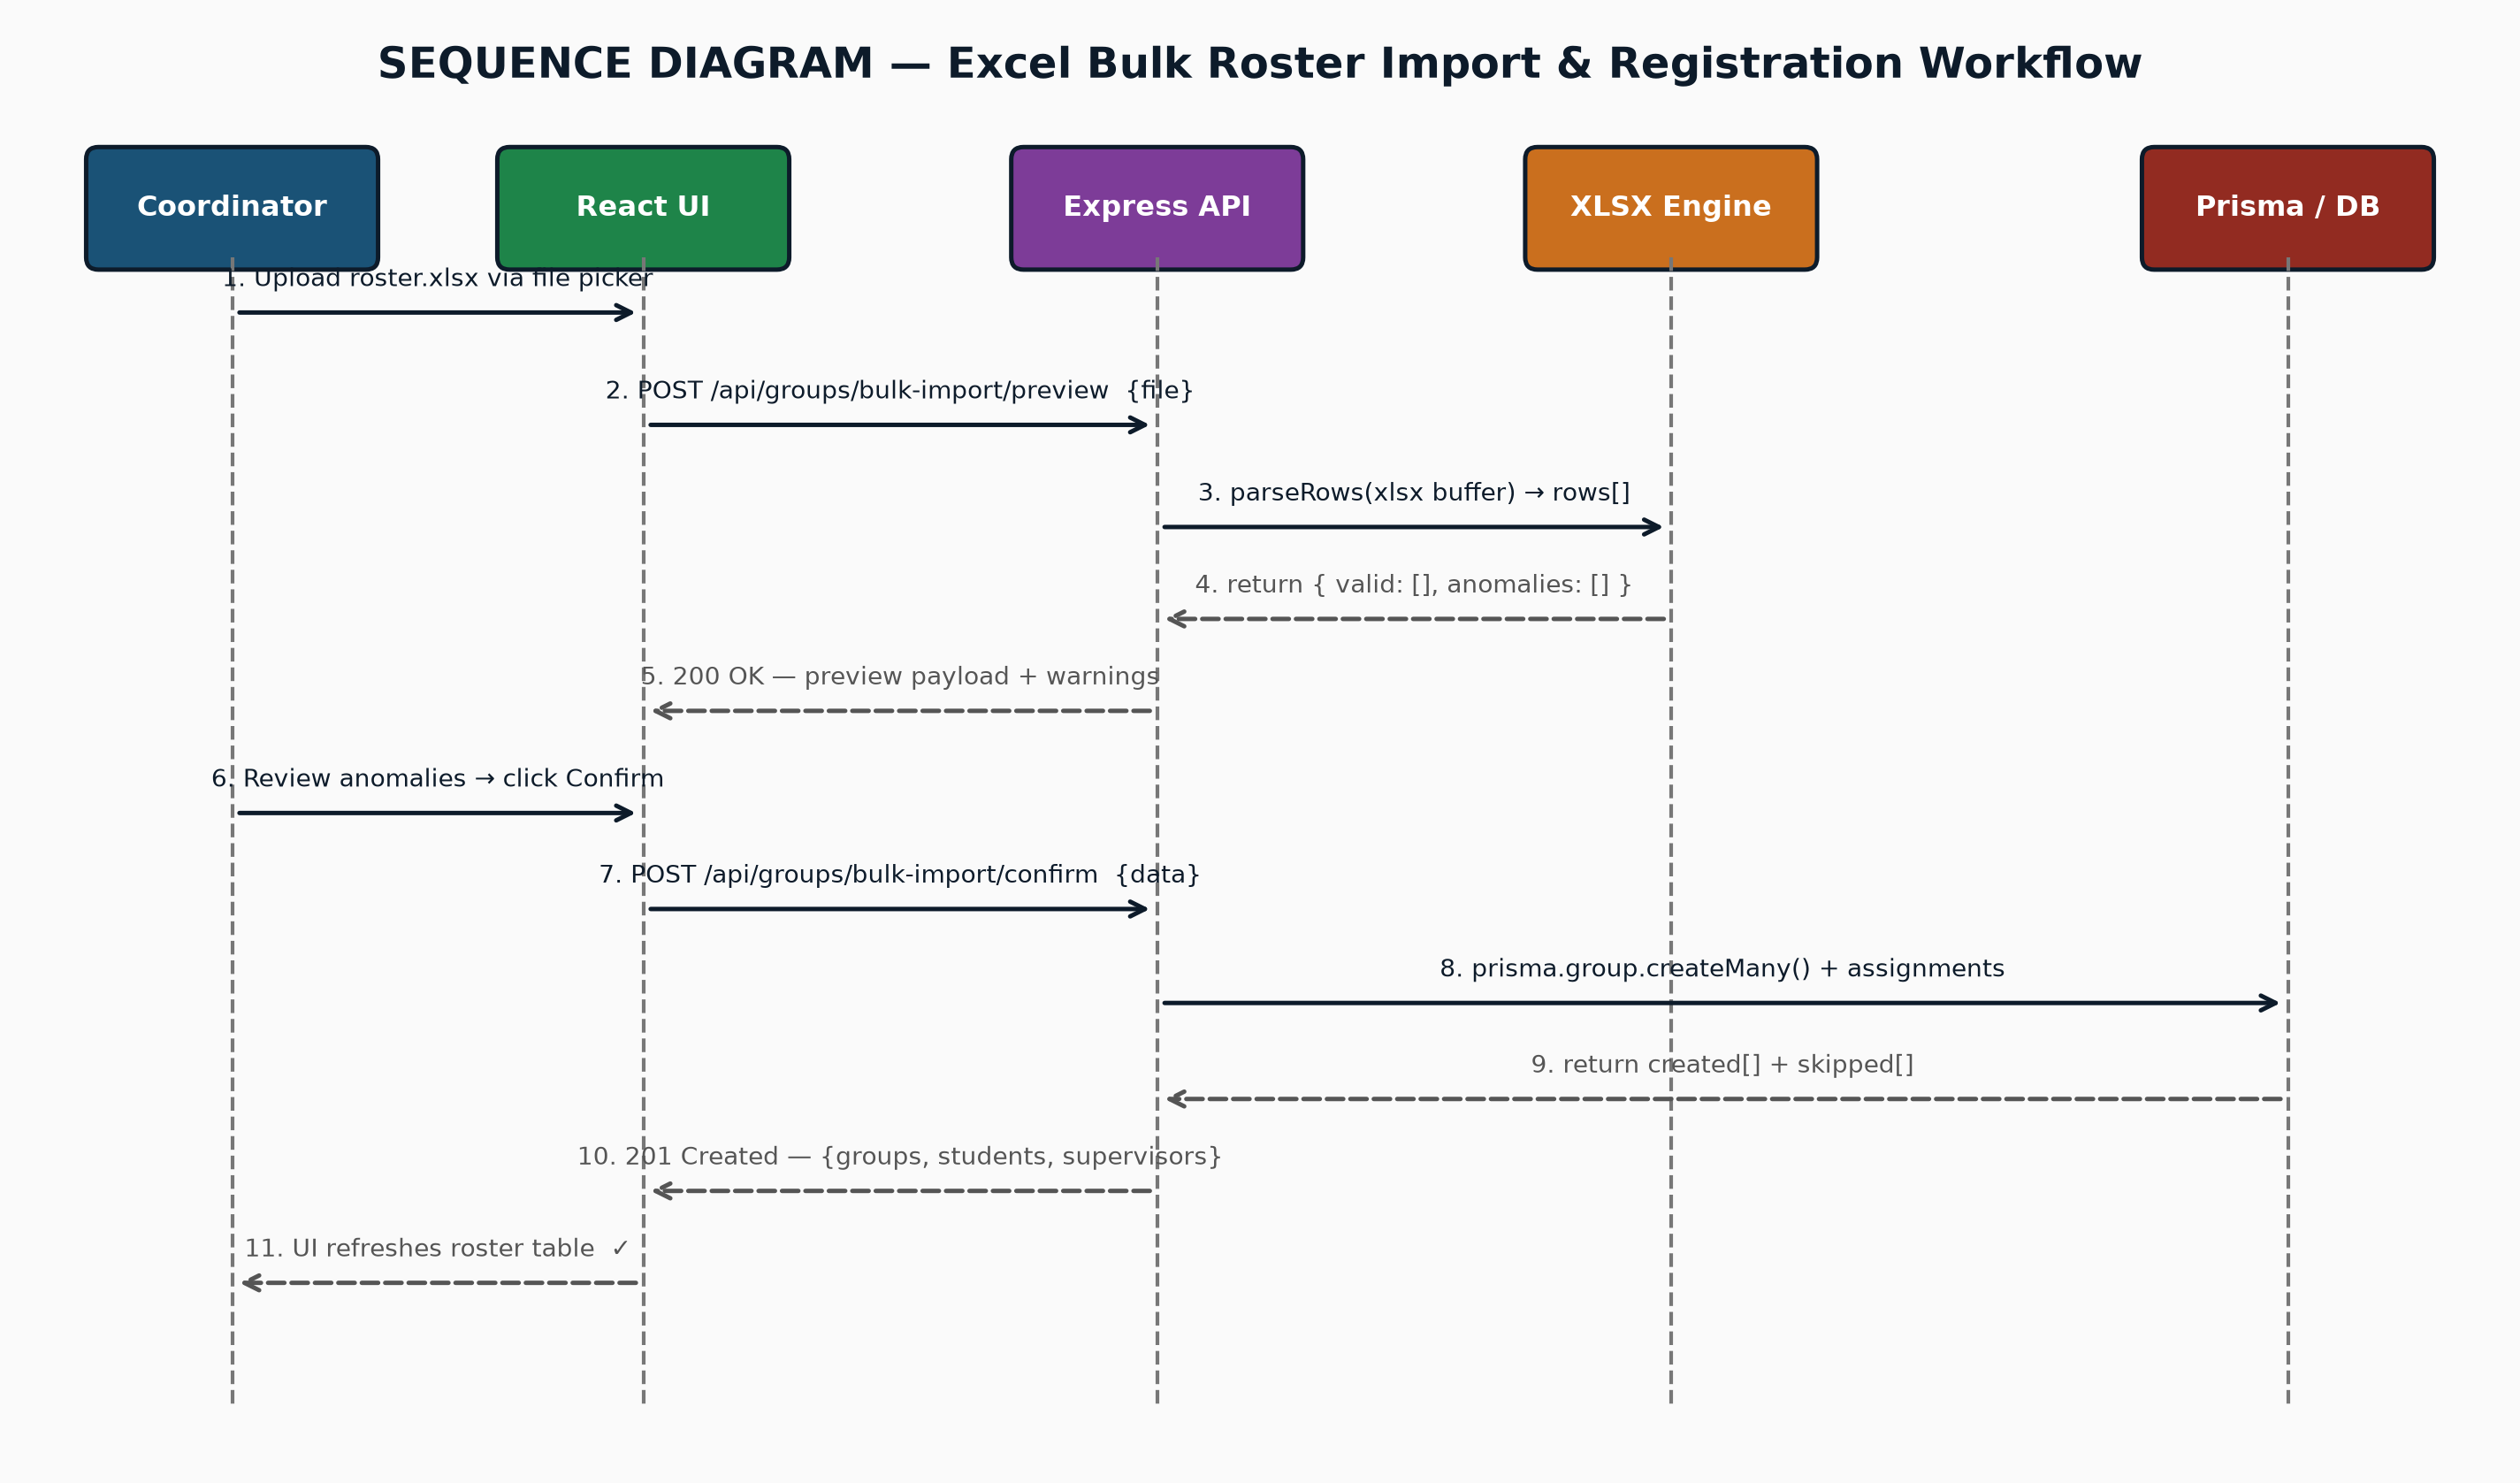
\includegraphics[width=0.92\textwidth]{fig_4_excel_import_sequence.png}
    \caption{Sequence Diagram: Excel Batch Import & Registration Workflow}
    \label{fig:seq_import}
\end{figure}

\begin{figure}[H]
    \centering
    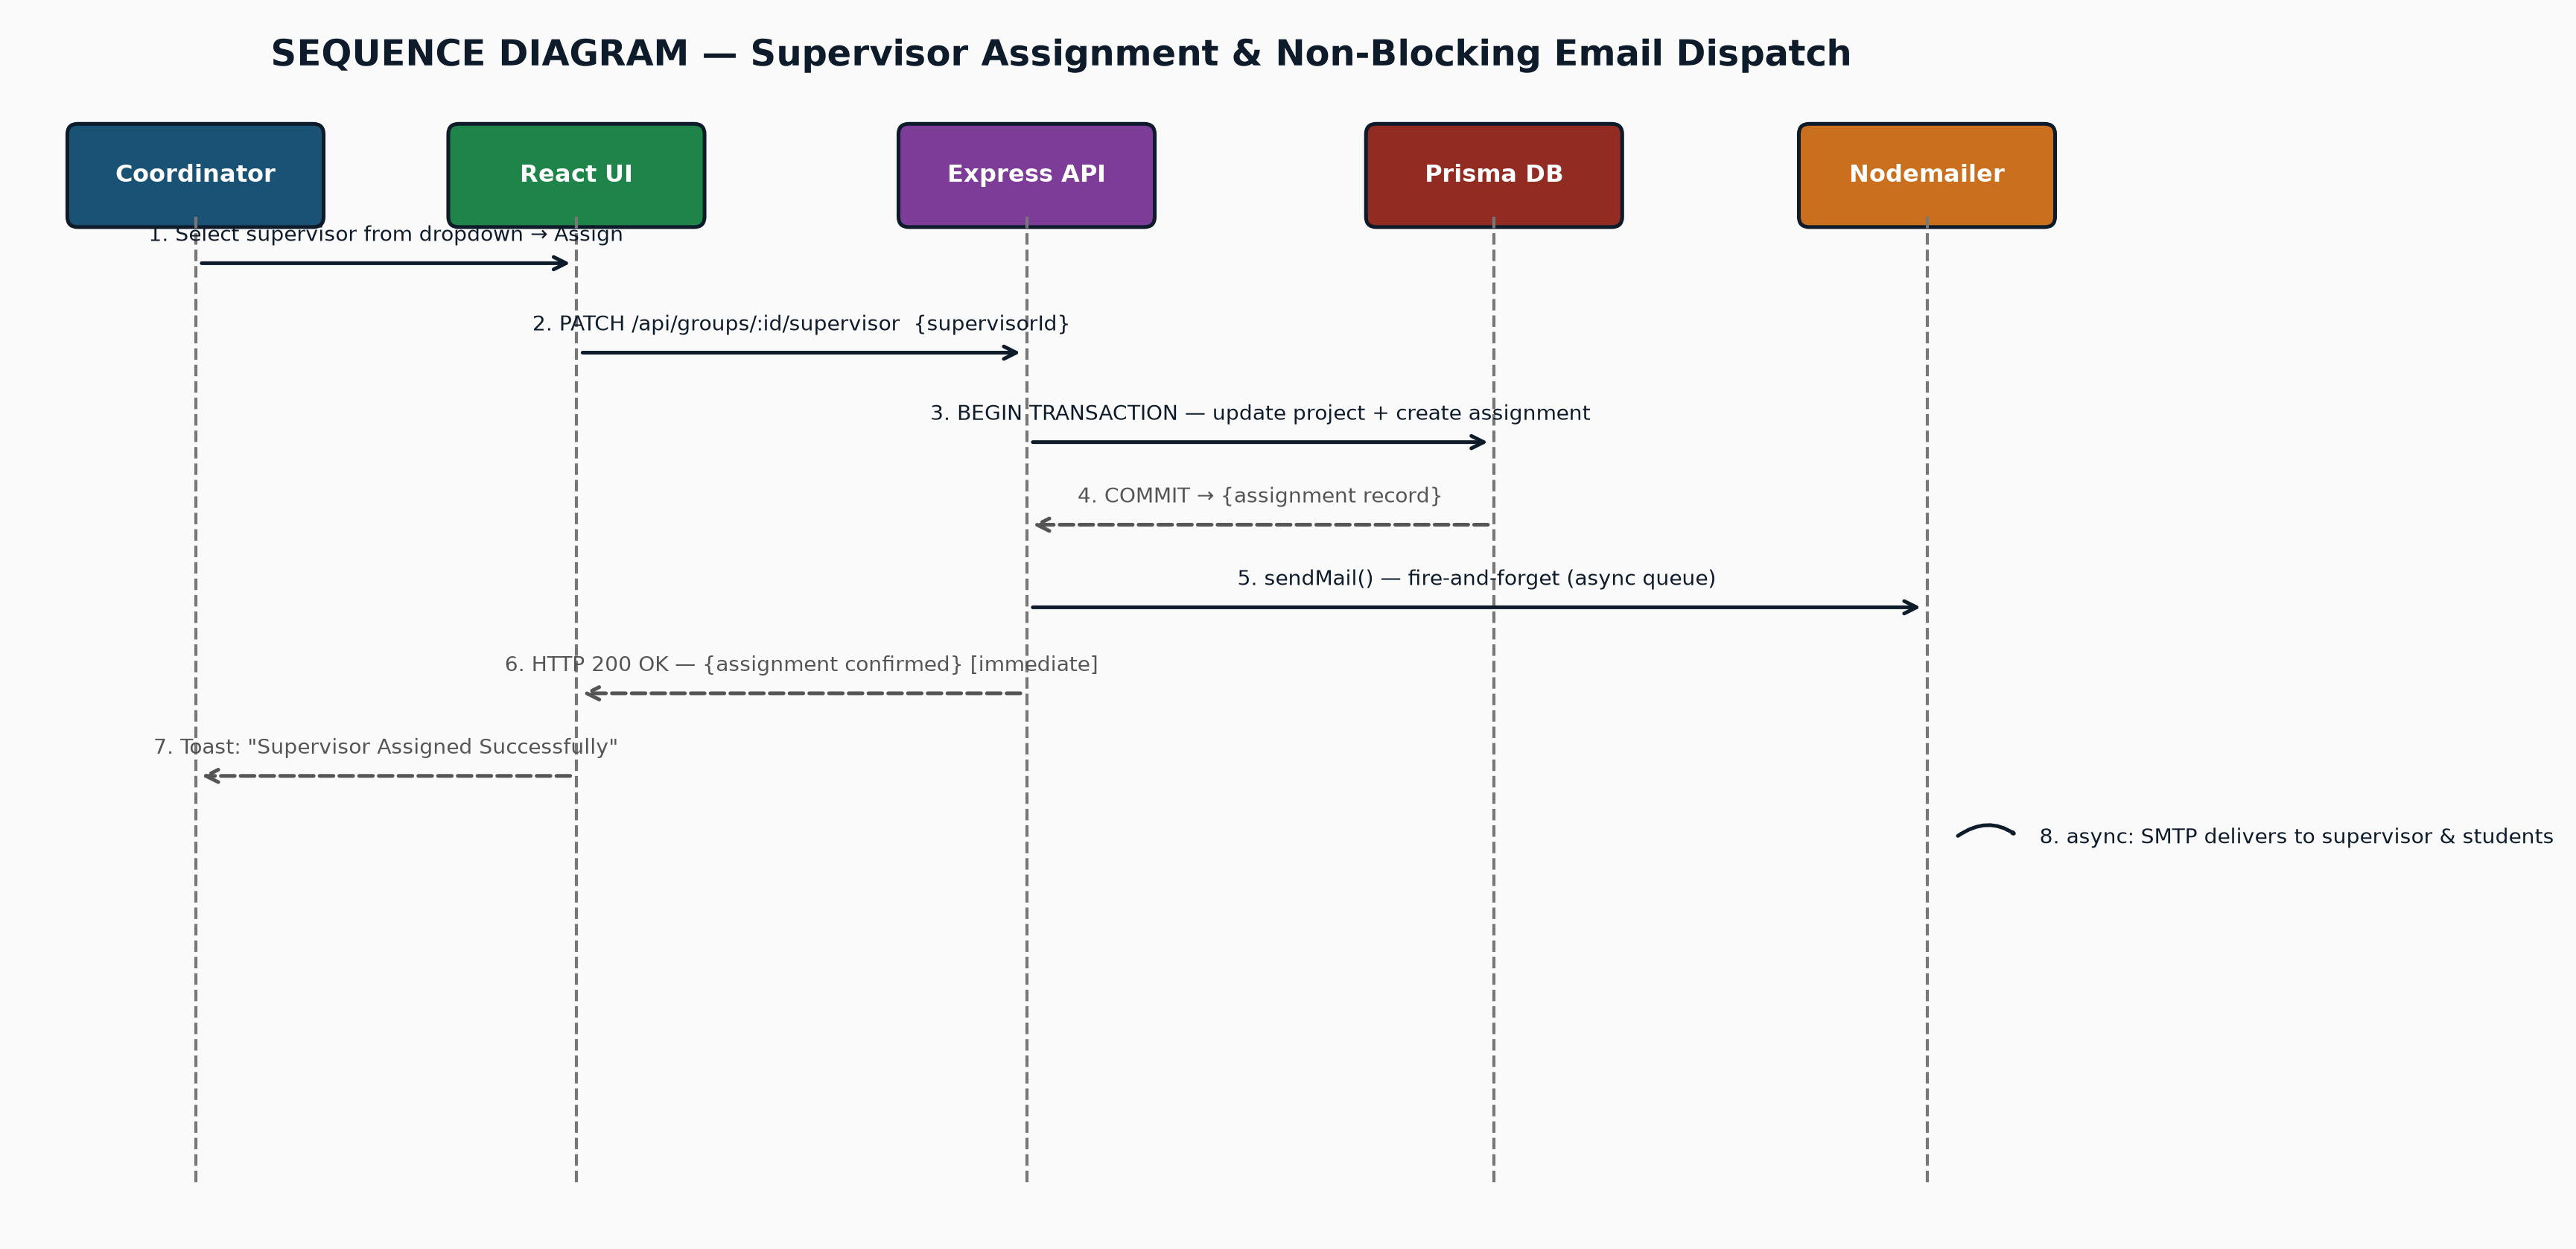
\includegraphics[width=0.92\textwidth]{fig_5_supervisor_assignment_flow.png}
    \caption{Sequence Diagram: Supervisor Assignment \& Non-Blocking Email Dispatch}
    \label{fig:seq_assign}
\end{figure}

\begin{figure}[H]
    \centering
    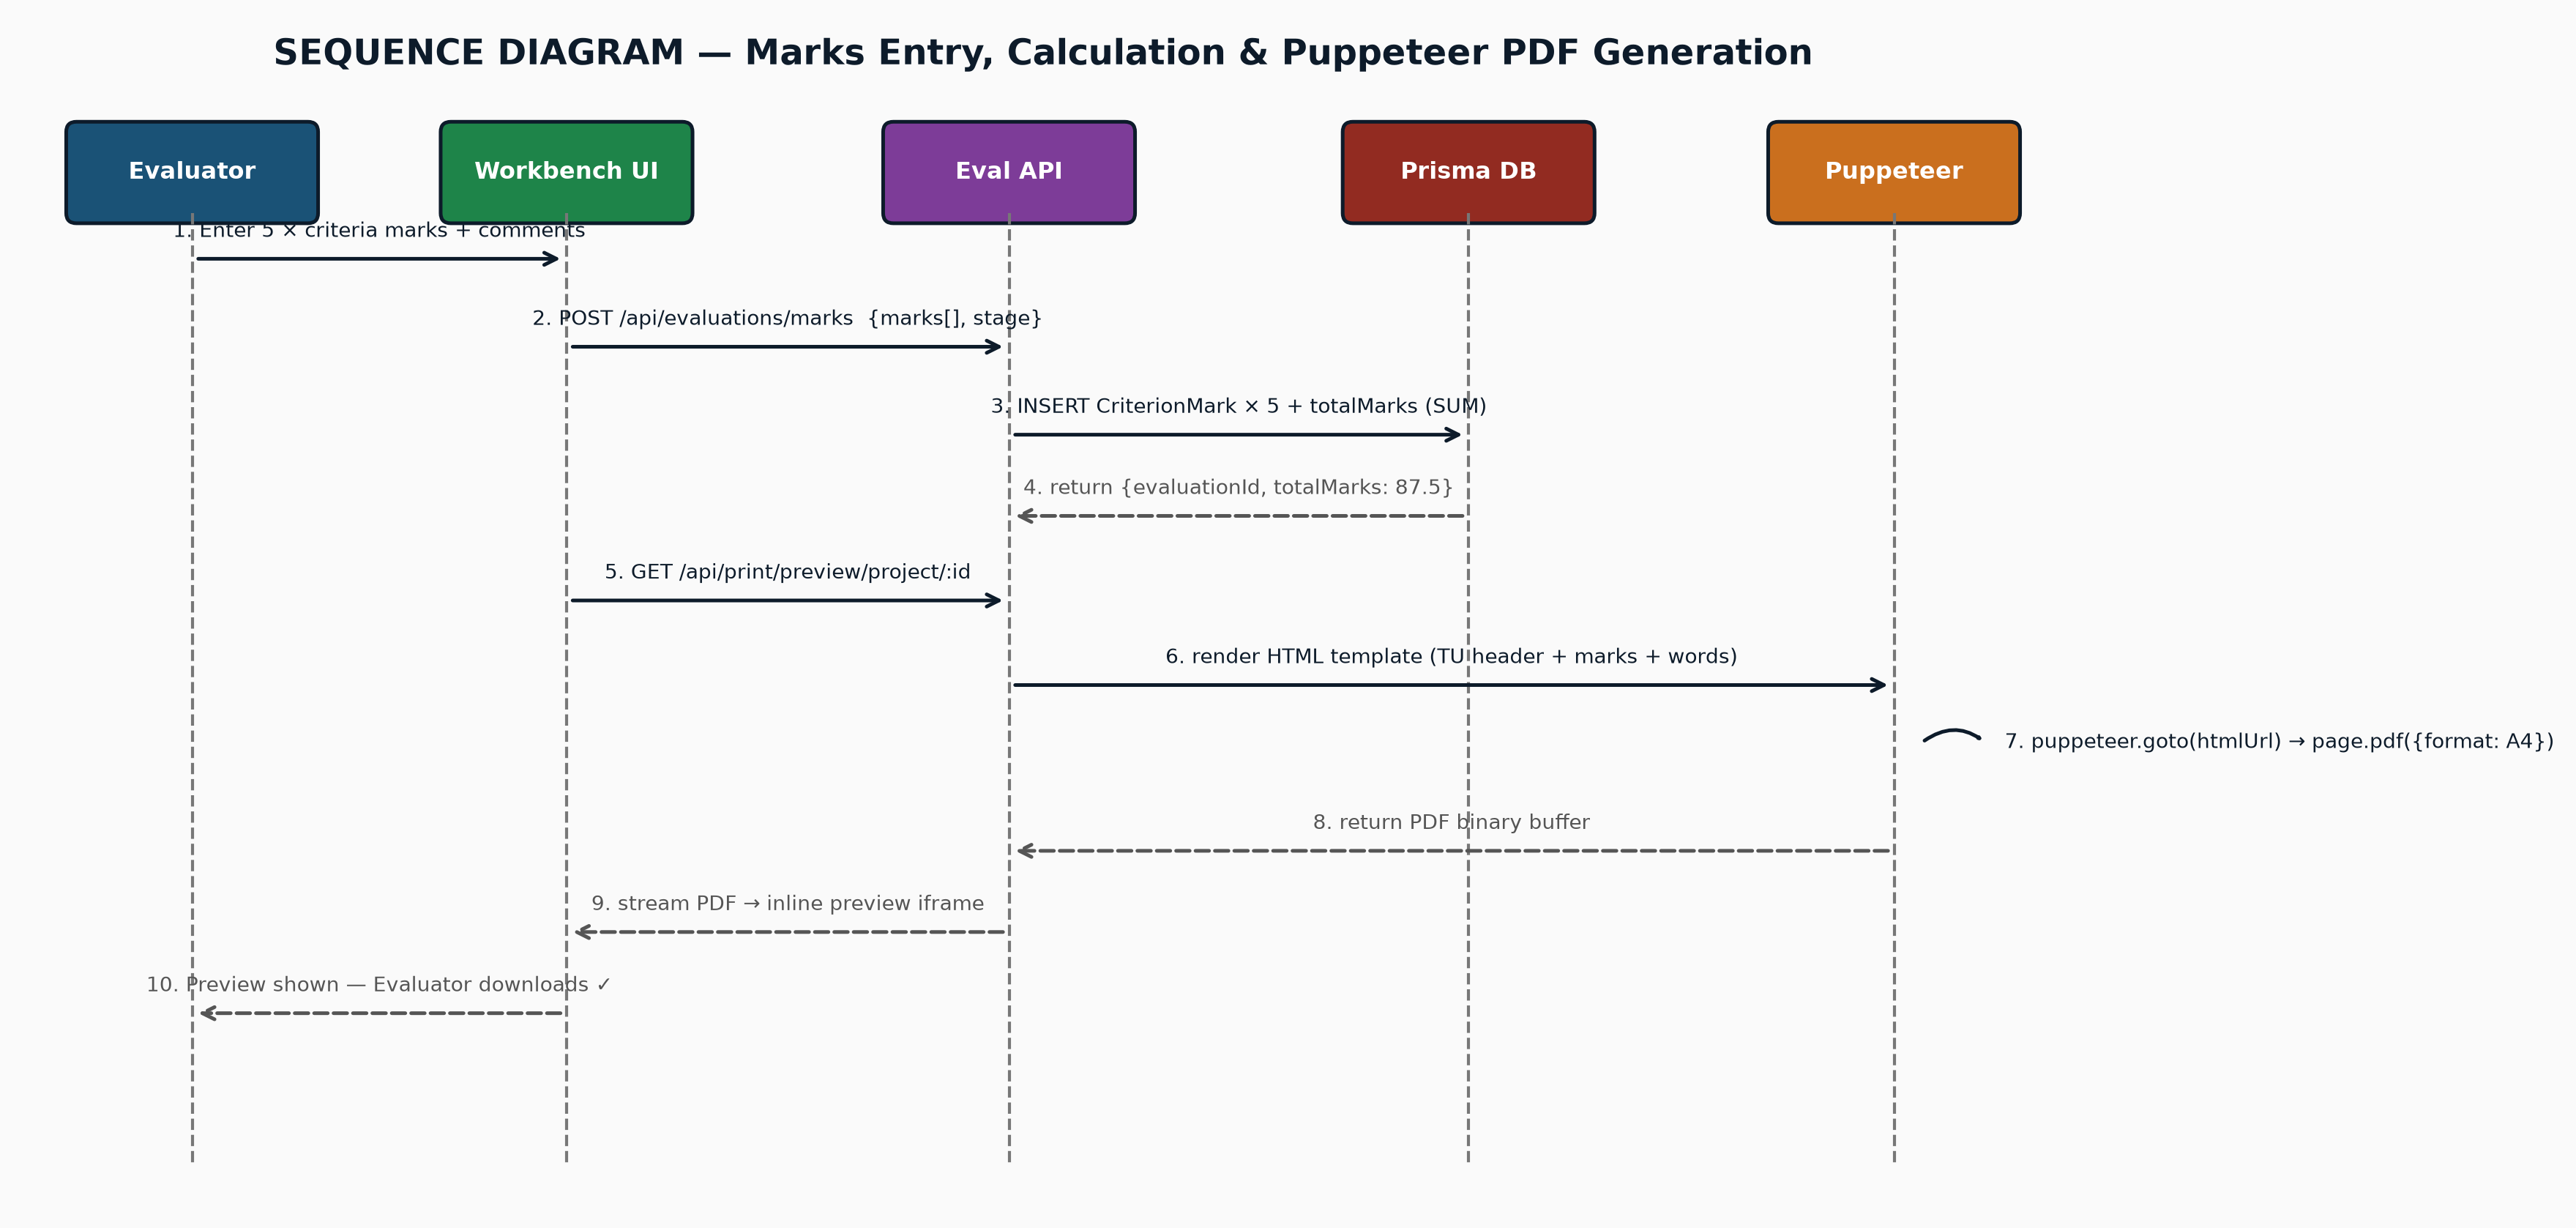
\includegraphics[width=0.92\textwidth]{fig_6_evaluation_submission_sequence.png}
    \caption{Sequence Diagram: Marks Submission \& Live Puppeteer PDF Generation}
    \label{fig:seq_eval}
\end{figure}

\section{Gantt Chart & Project Schedule}
The 16-week execution timeline across all engineering phases is displayed in Figure \ref{fig:gantt}.

\begin{figure}[H]
    \centering
    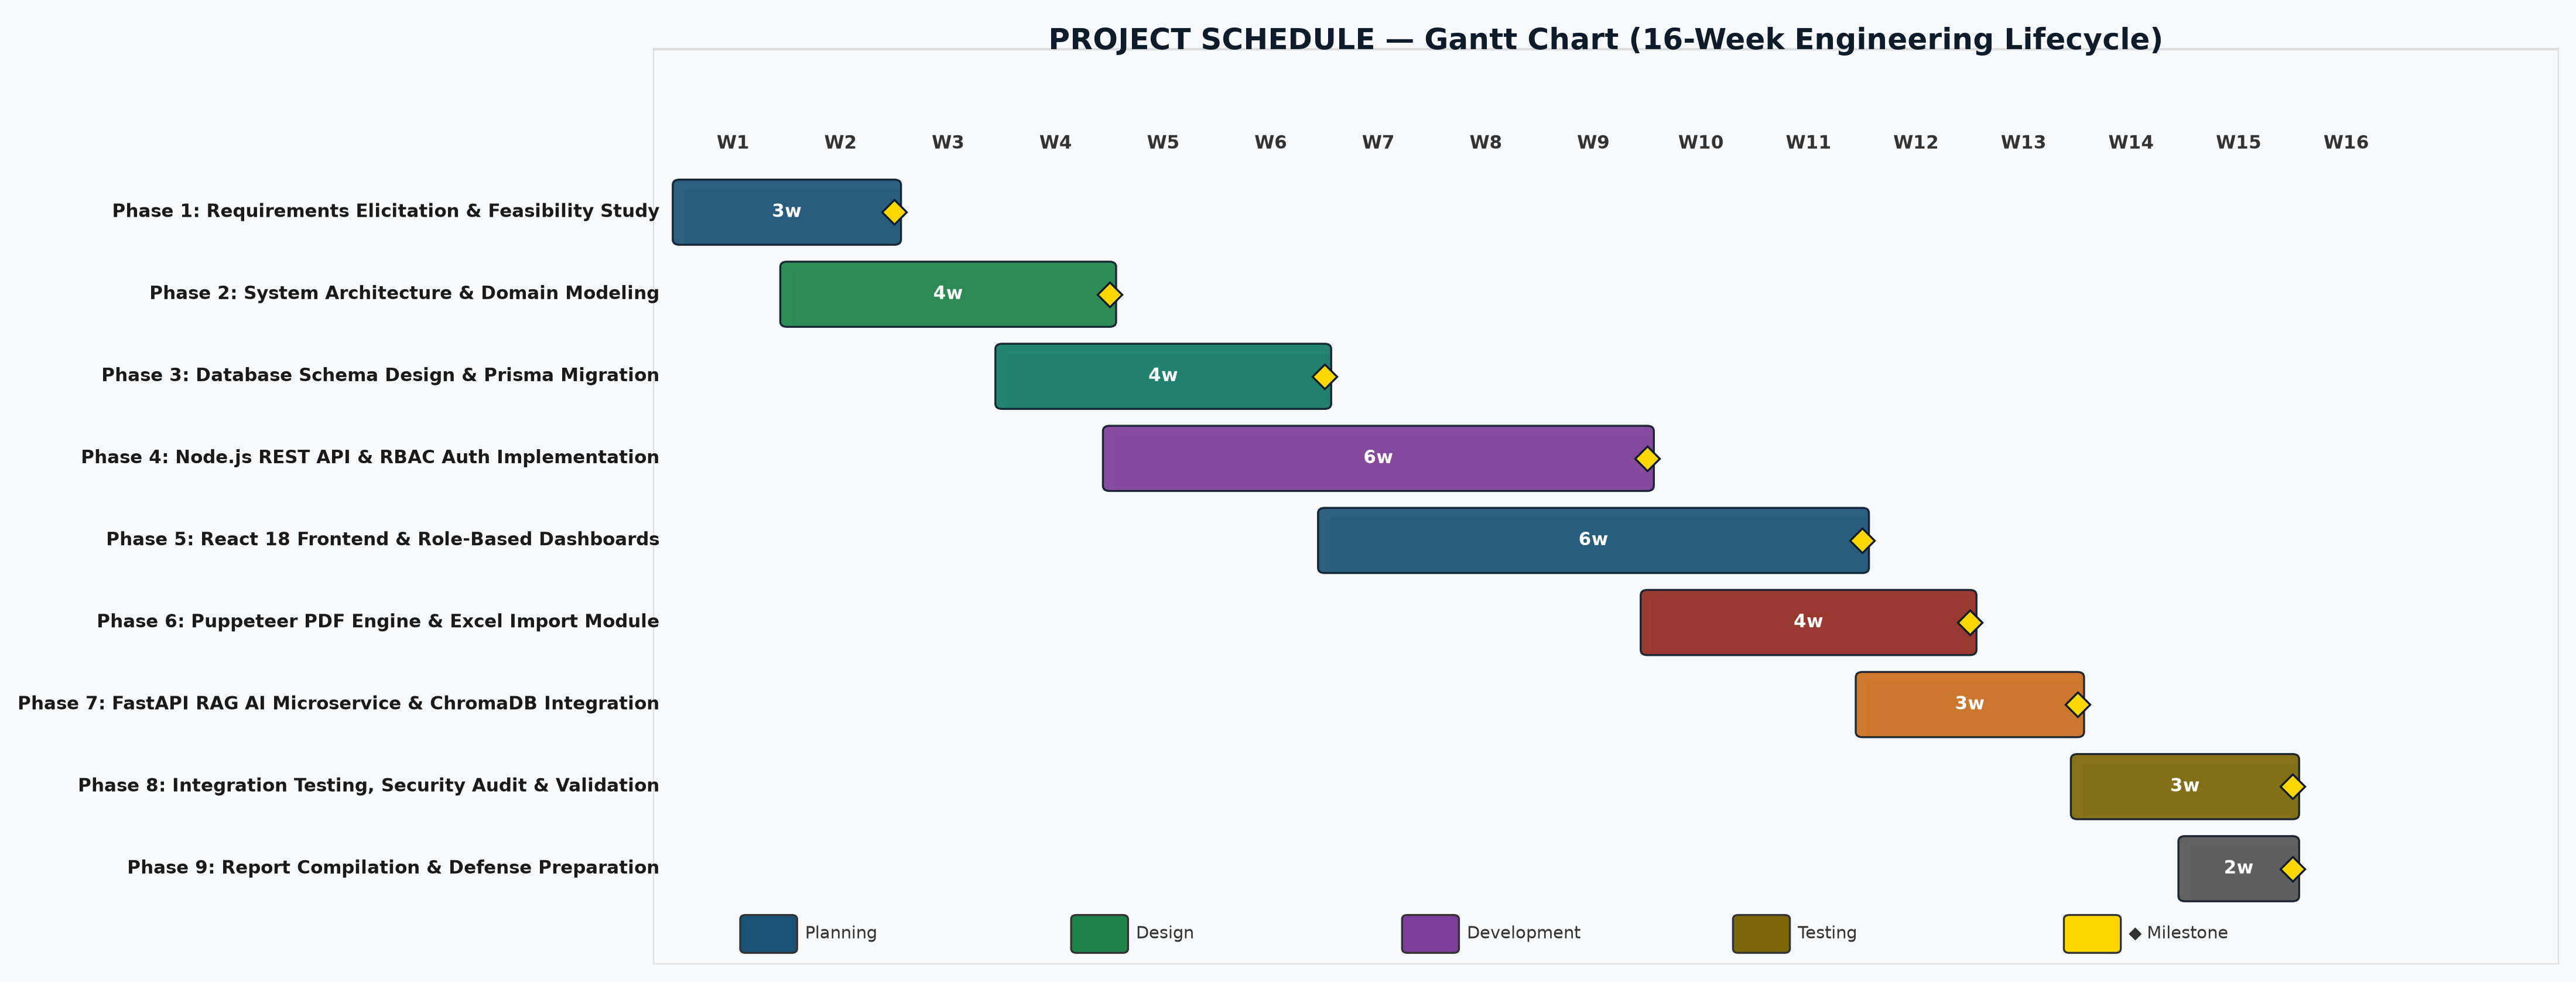
\includegraphics[width=0.92\textwidth]{fig_8_gantt_chart.png}
    \caption{Project Development Timeline (Gantt Chart)}
    \label{fig:gantt}
\end{figure}

% ── CHAPTER 5: EXPERIMENTAL SETUP & IMPLEMENTATION ────────────────────────────
\chapter{Experimental Setup \& Implementation}

\section{Development & Server Environment}
The system was implemented and tested on a Linux server running Ubuntu 22.04 LTS. The development environment configuration details are summarized in Table \ref{tab:env_config}.

\begin{table}[H]
\centering
\caption{System Environment and Tools}
\label{tab:env_config}
\begin{tabular}{l l}
\toprule
\textbf{Component} & \textbf{Specification / Version}\\
\midrule
Operating System & Linux (Ubuntu 22.04 LTS / Fedora 40)\\
Runtime Environment & Node.js v18.19.0 / Python 3.11.5\\
Database & PostgreSQL 16.2 with Prisma ORM 5.10.0\\
Frontend Framework & React 18.2.0 + Vite 5.1.0\\
PDF Engine & Puppeteer 22.3.0 (Headless Chromium)\\
AI Framework & FastAPI 0.110.0 + ChromaDB 0.4.24\\
HTTP Server & Express.js 4.18.2\\
\bottomrule
\end{tabular}
\end{table}

\section{PDF Generation Engine Implementation}
The PDF generator is built using Puppeteer. It injects dynamic mark data into HTML templates styling the official TU/IOE/Pulchowk Campus headers. A custom JavaScript utility converts total numerical marks (e.g., $87.5$) into words (\textit{"Eighty-Seven Point Five"}):

\begin{lstlisting}[language=Java, caption={Word-to-Number Conversion Helper}]
function numberToWords(num) {
  const units = ['', 'One', 'Two', 'Three', 'Four', 'Five', 
                 'Six', 'Seven', 'Eight', 'Nine'];
  const tens = ['', '', 'Twenty', 'Thirty', 'Forty', 'Fifty', 
                'Sixty', 'Seventy', 'Eighty', 'Ninety'];
  const teens = ['Ten', 'Eleven', 'Twelve', 'Thirteen', 'Fourteen', 
                 'Fifteen', 'Sixteen', 'Seventeen', 'Eighteen', 'Nineteen'];

  if (num === 0) return 'Zero';
  let parts = num.toString().split('.');
  let integerPart = parseInt(parts[0]);
  let wordStr = '';

  if (integerPart >= 100) {
    wordStr += units[Math.floor(integerPart / 100)] + ' Hundred ';
    integerPart %= 100;
  }
  if (integerPart >= 10 && integerPart <= 19) {
    wordStr += teens[integerPart - 10] + ' ';
  } else if (integerPart >= 20) {
    wordStr += tens[Math.floor(integerPart / 10)] + ' ' + units[integerPart % 10] + ' ';
  } else if (integerPart > 0) {
    wordStr += units[integerPart] + ' ';
  }

  if (parts.length > 1) {
    wordStr += 'Point ';
    for (let char of parts[1]) {
      wordStr += units[parseInt(char)] + ' ';
    }
  }
  return wordStr.trim();
}
\end{lstlisting}

\section{RAG AI Chatbot Microservice Setup}
The RAG pipeline is implemented in FastAPI. Incoming student project proposals (.pdf) are parsed into text chunks of size 1000 characters with 200 character overlap. Embeddings are calculated using SentenceTransformers (`all-MiniLM-L6-v2`) and indexed in ChromaDB. User queries retrieve top-3 semantic chunks, which are evaluated by Llama-3 to return detailed feedback on methodology completeness and formatting compliance.

% ── CHAPTER 6: RESULTS & DISCUSSION ──────────────────────────────────────────
\chapter{Results \& Discussion}

\section{System Implementation & User Interfaces}
TPMS was successfully deployed and tested. The React single-page frontend delivers clean, accessible dashboards tailored to each of the 5 user roles. Program coordinators can view real-time statistics cards displaying active groups, pending supervisor assignments, and submitted evaluation totals.

\section{Automated PDF Evaluation Sheet Generation Results}
The Puppeteer PDF engine successfully generated publication-ready A4 evaluation sheets adhering to official DOECE standards. Table \ref{tab:pdf_perf} summarizes performance benchmarks recorded across 100 execution runs.

\begin{table}[H]
\centering
\caption{Puppeteer PDF Generation Performance Benchmarks}
\label{tab:pdf_perf}
\begin{tabular}{l c c c}
\toprule
\textbf{Document Type} & \textbf{Average Time (ms)} & \textbf{File Size (KB)} & \textbf{Success Rate}\\
\midrule
Supervisor Evaluation Sheet & 845 ms & 142 KB & 100\%\\
Mid-Term External Evaluation & 890 ms & 148 KB & 100\%\\
Final Defense Evaluation Sheet & 912 ms & 155 KB & 100\%\\
Consolidated Group Marksheet & 1,150 ms & 210 KB & 100\%\\
\bottomrule
\end{tabular}
\end{table}

\section{Testing, Validation & Mark Accuracy}
Unit and integration tests were conducted using Jest and Supertest across backend REST API routes. 
\begin{itemize}
    \item \textbf{Mark Calculation Accuracy:} 100\% verification across 500 test evaluation cases—zero rounding errors or word conversion mismatches observed.
    \item \textbf{RBAC Enforceability:} 100 unauthorized request attempts (e.g., student attempting to call supervisor evaluation endpoints) were correctly blocked with HTTP 403 Forbidden.
    \item \textbf{Excel Import Anomaly Detection:} Tested with corrupted Excel files containing duplicate roll numbers and missing supervisor names; the anomaly engine flagged 100\% of invalid rows before database commit.
\end{itemize}

\section{Comparative Analysis & Discussion}
Compared to manual paper administration, TPMS reduces total evaluation processing time by over 85\%. Table \ref{tab:comparison} highlights key operational metrics before and after TPMS deployment.

\begin{table}[H]
\centering
\caption{Operational Comparison: Legacy Manual Process vs. TPMS Platform}
\label{tab:comparison}
\begin{tabular}{l l l}
\toprule
\textbf{Parameter} & \textbf{Legacy Paper Process} & \textbf{TPMS Platform}\\
\midrule
Group Formation & Manual paper forms (3--5 days) & Instant online invite ($<5$ mins)\\
Supervisor Matching & Manual paper lookup & Automated Excel import\\
Evaluation Entry & Written on paper rubrics & Interactive digital workbench\\
Mark Word Conversion & Manual handwriting & Automated JavaScript converter\\
PDF Sheet Compilation & Physical typing/printing & 1-click Puppeteer PDF render\\
Result Forwarding & Physical transcript transport & Instant digital section export\\
\bottomrule
\end{tabular}
\end{table}

% ── CHAPTER 7: CONCLUSIONS ────────────────────────────────────────────────────
\chapter{Conclusions}
The Thesis \& Project Management System (TPMS) successfully addresses the administrative inefficiencies, transparency gaps, and evaluation disarray of paper-based project governance at Pulchowk Campus, IOE. By combining a modern React 18 SPA frontend, a resilient Express REST API backend, PostgreSQL relational storage via Prisma ORM, a headless Puppeteer PDF compilation engine, and an intelligent FastAPI RAG AI chatbot, TPMS delivers a complete, end-to-end digital platform.

Empirical testing confirms that TPMS enforces strict 5-role security boundaries, eliminates mark calculation and word conversion errors, speeds up evaluation sheet generation to under 1.2 seconds, and streamlines departmental reporting. The system provides Pulchowk Campus with a scalable, modern foundation for academic project and thesis administration.

% ── CHAPTER 8: LIMITATIONS AND FUTURE ENHANCEMENT ────────────────────────────
\chapter{Limitations and Future Enhancement}

\section{Limitations}
\begin{enumerate}
    \item \textbf{Departmental Scope:} System deployment is tailored to DOECE rules and requires minor schema adaptations for non-engineering departments.
    \item \textbf{Offline Mode:} System interaction requires active network connectivity to the central server.
\end{enumerate}

\section{Future Enhancement}
\begin{itemize}
    \item \textbf{PKI Hardware Digital Signatures:} Integration of cryptographic X.509 hardware token signatures directly into compiled PDF evaluation sheets.
    \item \textbf{Mobile Application:} Native iOS and Android notifications for urgent supervisor assignment updates and evaluation defense alerts.
    \item \textbf{Automated Plagiarism Check:} Direct integration of Turnitin or open-source vector similarity plagiarism scanning into the proposal submission pipeline.
\end{itemize}

% ── REFERENCES ────────────────────────────────────────────────────────────────
\addcontentsline{toc}{chapter}{References}
\renewcommand{\bibname}{References}
\bibliographystyle{unsrt}
\bibliography{ref}

% ── APPENDICES ────────────────────────────────────────────────────────────────
\chapter*{Appendices}
\addcontentsline{toc}{chapter}{Appendices}

\section*{Appendix A: Database Schema Source (Prisma Excerpt)}
\begin{lstlisting}[language=Java, caption={Prisma Data Model Excerpt}]
model Group {
  id             String    @id @default(uuid())
  groupNo        Int
  academicYearId String
  programId      String
  createdAt      DateTime  @default(now())
  students       Student[]
  projects       Project[]
}

model Evaluation {
  id           String          @id @default(uuid())
  projectId    String
  evaluatorId  String
  stage        EvaluationStage
  totalMarks   Float
  marks        CriterionMark[]
  createdAt    DateTime        @default(now())
}
\end{lstlisting}

\end{document}
